\SourceLeaf{211}\Needspace{20\baselineskip}
Wir haben nun zwei Fälle zu unterscheiden.

I. Schneidet $AC\mathinner{.\,.\,.}$ die Linie $1$ in $D$, so mache man $BE = BD$, indem

\begin{center}
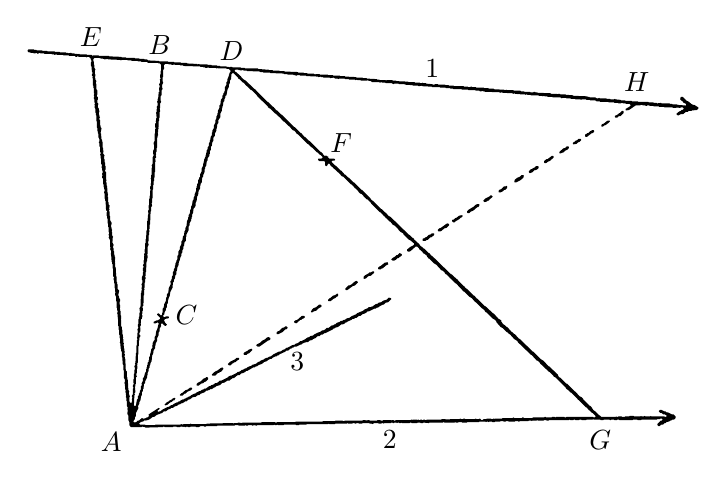
\begin{tikzpicture}[x=0.00642066cm,y=-0.00642066cm]
\fill[even odd rule] (814,424) -- (813,423) -- (809,423) -- (807,425) -- (803,426) -- (799,430) -- (796,431) -- (794,433) -- (792,433) -- (791,434) -- (791,437) -- (792,438) -- (796,438) -- (799,436) -- (801,436) -- (806,431) -- (808,431) -- (810,429) -- (811,429) -- (813,427) -- cycle
(843,405) -- (841,403) -- (838,404) -- (827,412) -- (824,413) -- (821,416) -- (821,418) -- (822,419) -- (826,419) -- (828,418) -- (834,413) -- (838,412) -- (843,407) -- cycle
(870,388) -- (869,387) -- (863,388) -- (858,392) -- (855,393) -- (852,396) -- (850,396) -- (849,397) -- (849,399) -- (851,401) -- (854,401) -- (856,399) -- (863,395) -- (866,392) -- (867,392) -- (870,389) -- cycle
(903,366) -- (902,365) -- (899,365) -- (895,367) -- (892,370) -- (882,376) -- (879,379) -- (879,382) -- (880,383) -- (883,383) -- (886,380) -- (891,378) -- (899,371) -- (901,371) -- (903,368) -- cycle
(929,350) -- (927,348) -- (925,348) -- (923,350) -- (915,354) -- (911,358) -- (911,359) -- (913,361) -- (918,360) -- (920,358) -- (922,358) -- (923,356) -- (929,351) -- cycle
(958,330) -- (957,329) -- (955,330) -- (952,330) -- (946,336) -- (944,336) -- (941,339) -- (941,341) -- (942,342) -- (945,342) -- (949,340) -- (952,337) -- (954,337) -- (958,333) -- cycle
(991,309) -- (990,308) -- (986,308) -- (983,311) -- (978,313) -- (973,317) -- (972,321) -- (973,322) -- (976,322) -- (984,318) -- (990,313) -- cycle
(1020,291) -- (1019,290) -- (1015,290) -- (1012,293) -- (1009,294) -- (1007,296) -- (1005,296) -- (1001,300) -- (1001,302) -- (1003,304) -- (1008,302) -- (1012,298) -- (1014,298) -- (1018,296) -- (1020,294) -- cycle
(1050,271) -- (1049,270) -- (1046,270) -- (1038,276) -- (1036,276) -- (1031,280) -- (1031,283) -- (1032,284) -- (1035,284) -- (1039,281) -- (1042,280) -- (1050,273) -- cycle
(1080,252) -- (1079,251) -- (1076,251) -- (1073,254) -- (1069,255) -- (1061,262) -- (1061,264) -- (1062,265) -- (1064,265) -- (1065,264) -- (1069,263) -- (1072,260) -- (1078,257) -- (1080,254) -- cycle
(1104,237) -- (1103,236) -- (1099,236) -- (1096,239) -- (1094,239) -- (1091,242) -- (1090,242) -- (1088,244) -- (1088,246) -- (1089,247) -- (1095,246) -- (1098,243) -- (1101,242) -- (1104,239) -- cycle
(1130,220) -- (1129,219) -- (1126,219) -- (1122,221) -- (1118,225) -- (1116,225) -- (1114,227) -- (1113,227) -- (1112,228) -- (1112,231) -- (1113,232) -- (1116,232) -- (1125,225) -- (1127,225) -- (1130,222) -- cycle
(1161,201) -- (1160,200) -- (1157,200) -- (1155,201) -- (1149,206) -- (1146,207) -- (1144,209) -- (1144,211) -- (1145,212) -- (1147,212) -- (1151,209) -- (1153,209) -- (1156,206) -- (1157,206) -- (1161,202) -- cycle
(1188,182) -- (1187,181) -- (1185,181) -- (1181,185) -- (1180,185) -- (1175,189) -- (1172,190) -- (1171,191) -- (1171,193) -- (1172,194) -- (1176,194) -- (1179,191) -- (1182,191) -- (1188,185) -- cycle
(10,61) -- (10,63) -- (12,65) -- (15,65) -- (16,66) -- (21,66) -- (22,67) -- (25,67) -- (27,66) -- (30,68) -- (34,66) -- (35,67) -- (42,67) -- (43,68) -- (57,68) -- (58,69) -- (62,69) -- (63,70) -- (67,69) -- (68,70) -- (80,70) -- (81,71) -- (91,71) -- (92,72) -- (103,72) -- (105,74) -- (107,74) -- (108,73) -- (110,73) -- (111,74) -- (125,74) -- (126,75) -- (128,74) -- (131,74) -- (135,78) -- (135,80) -- (136,81) -- (136,84) -- (135,85) -- (135,91) -- (136,92) -- (137,103) -- (138,104) -- (138,108) -- (137,109) -- (137,111) -- (139,113) -- (138,115) -- (139,117) -- (139,130) -- (140,131) -- (140,135) -- (141,136) -- (141,146) -- (142,147) -- (141,149) -- (141,151) -- (142,152) -- (141,154) -- (141,157) -- (142,158) -- (142,164) -- (143,165) -- (143,167) -- (142,168) -- (143,171) -- (142,173) -- (144,177) -- (144,184) -- (145,185) -- (145,189) -- (146,190) -- (146,201) -- (147,202) -- (147,214) -- (148,215) -- (148,221) -- (149,222) -- (149,225) -- (150,226) -- (150,233) -- (152,237) -- (152,241) -- (151,242) -- (151,244) -- (152,245) -- (152,251) -- (153,252) -- (153,262) -- (155,264) -- (153,268) -- (154,269) -- (154,274) -- (155,275) -- (155,285) -- (157,288) -- (156,293) -- (157,294) -- (157,298) -- (158,299) -- (158,304) -- (157,305) -- (158,309) -- (157,310) -- (157,313) -- (159,315) -- (159,325) -- (160,326) -- (160,331) -- (161,332) -- (161,335) -- (162,336) -- (162,340) -- (161,341) -- (161,343) -- (162,344) -- (162,354) -- (163,355) -- (163,358) -- (164,359) -- (165,377) -- (167,379) -- (167,381) -- (166,382) -- (166,388) -- (167,389) -- (167,393) -- (168,394) -- (168,403) -- (169,404) -- (169,410) -- (170,411) -- (170,420) -- (171,421) -- (171,424) -- (170,425) -- (171,429) -- (170,431) -- (173,437) -- (173,450) -- (174,451) -- (173,454) -- (175,458) -- (175,462) -- (174,464) -- (175,465) -- (176,479) -- (177,480) -- (177,483) -- (178,484) -- (178,492) -- (179,493) -- (179,508) -- (181,510) -- (180,512) -- (180,515) -- (181,516) -- (181,521) -- (182,522) -- (182,531) -- (183,532) -- (183,538) -- (184,539) -- (183,541) -- (183,545) -- (185,549) -- (185,557) -- (186,558) -- (186,570) -- (187,571) -- (187,575) -- (188,576) -- (187,582) -- (188,583) -- (188,589) -- (189,590) -- (188,592) -- (189,594) -- (189,606) -- (190,607) -- (190,613) -- (191,614) -- (191,623) -- (192,624) -- (192,630) -- (193,631) -- (193,637) -- (192,639) -- (193,640) -- (194,651) -- (195,652) -- (195,656) -- (196,657) -- (196,667) -- (197,668) -- (198,682) -- (199,683) -- (199,693) -- (200,694) -- (200,708) -- (202,712) -- (202,717) -- (201,719) -- (202,720) -- (203,732) -- (204,733) -- (203,737) -- (204,738) -- (204,742) -- (205,743) -- (204,747) -- (205,748) -- (205,754) -- (206,755) -- (206,764) -- (208,768) -- (207,770) -- (208,772) -- (207,780) -- (209,783) -- (209,792) -- (211,796) -- (211,802) -- (214,806) -- (235,806) -- (236,805) -- (242,806) -- (243,807) -- (277,806) -- (278,805) -- (280,805) -- (281,806) -- (297,806) -- (298,805) -- (304,805) -- (305,806) -- (311,806) -- (312,805) -- (316,805) -- (317,806) -- (319,805) -- (321,806) -- (323,806) -- (324,805) -- (326,805) -- (327,806) -- (331,806) -- (332,805) -- (342,805) -- (343,806) -- (348,806) -- (352,804) -- (358,804) -- (359,805) -- (362,805) -- (363,804) -- (384,804) -- (385,803) -- (419,803) -- (420,802) -- (426,802) -- (427,803) -- (439,803) -- (440,802) -- (442,803) -- (445,803) -- (446,802) -- (453,802) -- (454,803) -- (460,802) -- (461,803) -- (463,803) -- (464,802) -- (496,802) -- (497,801) -- (499,802) -- (502,802) -- (503,801) -- (505,802) -- (516,802) -- (517,801) -- (540,801) -- (541,802) -- (546,802) -- (547,801) -- (561,801) -- (562,800) -- (604,800) -- (605,799) -- (607,800) -- (617,800) -- (618,799) -- (641,799) -- (642,798) -- (644,799) -- (652,799) -- (653,798) -- (656,798) -- (657,799) -- (659,799) -- (660,798) -- (664,798) -- (665,799) -- (671,799) -- (672,798) -- (685,798) -- (686,799) -- (690,799) -- (692,800) -- (695,798) -- (703,798) -- (704,799) -- (709,799) -- (710,798) -- (712,798) -- (714,799) -- (715,798) -- (728,798) -- (729,797) -- (731,797) -- (732,798) -- (734,798) -- (735,797) -- (739,797) -- (740,798) -- (742,797) -- (744,797) -- (745,798) -- (747,798) -- (748,797) -- (750,798) -- (765,798) -- (766,797) -- (768,797) -- (769,798) -- (780,798) -- (781,797) -- (786,797) -- (787,798) -- (791,798) -- (792,797) -- (803,798) -- (804,797) -- (831,797) -- (832,796) -- (834,797) -- (854,797) -- (855,796) -- (857,797) -- (861,797) -- (862,796) -- (868,796) -- (869,797) -- (878,797) -- (879,796) -- (902,796) -- (903,795) -- (915,795) -- (916,796) -- (918,795) -- (920,795) -- (921,796) -- (923,795) -- (928,795) -- (929,796) -- (933,796) -- (934,795) -- (944,795) -- (945,794) -- (950,794) -- (951,795) -- (955,795) -- (956,794) -- (960,794) -- (961,795) -- (973,795) -- (974,794) -- (979,794) -- (980,795) -- (982,795) -- (983,794) -- (1000,794) -- (1001,793) -- (1005,793) -- (1007,794) -- (1008,793) -- (1016,793) -- (1017,792) -- (1019,793) -- (1030,793) -- (1031,792) -- (1035,792) -- (1036,793) -- (1040,793) -- (1041,792) -- (1080,792) -- (1081,791) -- (1083,792) -- (1089,792) -- (1090,791) -- (1092,791) -- (1093,792) -- (1100,792) -- (1101,791) -- (1104,791) -- (1105,792) -- (1114,792) -- (1115,791) -- (1127,791) -- (1128,790) -- (1129,791) -- (1142,791) -- (1143,792) -- (1148,792) -- (1149,791) -- (1160,791) -- (1161,792) -- (1163,792) -- (1164,791) -- (1169,791) -- (1170,792) -- (1175,792) -- (1176,791) -- (1179,791) -- (1180,792) -- (1206,792) -- (1207,791) -- (1215,791) -- (1216,792) -- (1223,792) -- (1224,791) -- (1254,791) -- (1255,790) -- (1260,790) -- (1261,789) -- (1264,789) -- (1265,790) -- (1265,792) -- (1264,793) -- (1262,793) -- (1255,800) -- (1255,802) -- (1257,804) -- (1259,804) -- (1263,801) -- (1266,801) -- (1269,798) -- (1271,798) -- (1273,796) -- (1278,795) -- (1280,793) -- (1282,793) -- (1285,791) -- (1288,791) -- (1291,788) -- (1291,785) -- (1287,781) -- (1284,781) -- (1276,777) -- (1273,777) -- (1271,775) -- (1269,775) -- (1263,772) -- (1260,772) -- (1258,774) -- (1258,775) -- (1261,778) -- (1263,778) -- (1267,781) -- (1270,781) -- (1273,783) -- (1273,785) -- (1272,786) -- (1270,786) -- (1269,785) -- (1243,785) -- (1242,784) -- (1240,785) -- (1231,785) -- (1230,784) -- (1228,785) -- (1224,785) -- (1223,784) -- (1221,785) -- (1209,785) -- (1208,784) -- (1200,784) -- (1199,785) -- (1191,785) -- (1190,786) -- (1185,786) -- (1184,785) -- (1178,785) -- (1177,786) -- (1175,786) -- (1174,785) -- (1172,786) -- (1144,786) -- (1141,783) -- (1140,783) -- (1131,774) -- (1130,774) -- (1128,772) -- (1125,767) -- (1122,764) -- (1121,764) -- (1108,751) -- (1108,750) -- (1105,747) -- (1101,745) -- (1093,736) -- (1092,736) -- (1076,720) -- (1075,720) -- (1063,708) -- (1062,708) -- (1059,705) -- (1058,702) -- (1041,686) -- (1040,686) -- (1030,675) -- (1025,672) -- (1010,657) -- (1009,657) -- (982,631) -- (981,631) -- (973,622) -- (972,622) -- (968,618) -- (967,618) -- (958,608) -- (957,608) -- (953,604) -- (952,604) -- (948,600) -- (948,599) -- (946,597) -- (947,596) -- (945,594) -- (941,592) -- (931,581) -- (930,581) -- (915,567) -- (914,567) -- (899,552) -- (898,552) -- (893,546) -- (892,546) -- (878,532) -- (877,532) -- (874,529) -- (874,528) -- (872,527) -- (861,516) -- (860,514) -- (859,514) -- (847,503) -- (846,503) -- (809,467) -- (808,467) -- (804,462) -- (803,462) -- (794,453) -- (793,453) -- (789,449) -- (788,449) -- (785,446) -- (785,445) -- (774,435) -- (774,434) -- (772,432) -- (771,432) -- (765,426) -- (764,426) -- (728,391) -- (723,388) -- (718,382) -- (717,382) -- (710,375) -- (709,375) -- (692,358) -- (691,358) -- (688,355) -- (688,354) -- (671,337) -- (670,337) -- (655,322) -- (654,322) -- (645,313) -- (644,313) -- (638,307) -- (637,307) -- (630,299) -- (629,299) -- (619,289) -- (618,289) -- (611,282) -- (611,281) -- (613,279) -- (616,279) -- (618,278) -- (617,276) -- (615,275) -- (606,275) -- (604,273) -- (604,270) -- (603,271) -- (602,271) -- (600,269) -- (597,270) -- (594,267) -- (594,266) -- (590,262) -- (589,262) -- (567,240) -- (566,240) -- (558,232) -- (557,232) -- (551,225) -- (550,225) -- (538,213) -- (537,213) -- (512,188) -- (511,188) -- (503,180) -- (502,180) -- (496,173) -- (495,173) -- (485,163) -- (484,163) -- (462,141) -- (461,139) -- (460,139) -- (441,121) -- (436,118) -- (432,114) -- (432,113) -- (422,104) -- (421,104) -- (419,102) -- (419,101) -- (421,99) -- (426,99) -- (427,100) -- (430,100) -- (431,101) -- (436,100) -- (437,101) -- (443,101) -- (444,102) -- (469,103) -- (470,104) -- (475,104) -- (476,105) -- (489,105) -- (490,106) -- (516,107) -- (517,108) -- (523,108) -- (524,109) -- (535,109) -- (536,110) -- (539,110) -- (540,111) -- (542,111) -- (543,110) -- (548,110) -- (549,111) -- (560,111) -- (561,112) -- (584,113) -- (585,114) -- (589,113) -- (590,114) -- (594,114) -- (595,115) -- (607,115) -- (608,116) -- (615,115) -- (618,117) -- (623,117) -- (624,118) -- (626,117) -- (637,117) -- (638,118) -- (645,118) -- (646,119) -- (657,119) -- (658,120) -- (661,119) -- (662,120) -- (668,120) -- (669,121) -- (680,121) -- (682,120) -- (683,121) -- (689,122) -- (691,124) -- (705,124) -- (706,125) -- (710,124) -- (711,125) -- (717,125) -- (718,126) -- (730,126) -- (733,128) -- (735,127) -- (743,127) -- (744,128) -- (755,128) -- (756,129) -- (771,130) -- (772,131) -- (782,131) -- (783,132) -- (789,131) -- (790,132) -- (809,133) -- (810,134) -- (825,134) -- (826,135) -- (836,135) -- (837,136) -- (845,136) -- (846,137) -- (851,137) -- (852,138) -- (868,138) -- (869,139) -- (881,139) -- (882,140) -- (895,140) -- (896,141) -- (903,141) -- (904,142) -- (907,142) -- (909,141) -- (910,142) -- (913,142) -- (914,143) -- (943,144) -- (944,145) -- (948,144) -- (949,145) -- (969,146) -- (970,147) -- (973,146) -- (974,147) -- (978,147) -- (979,148) -- (982,147) -- (983,148) -- (993,148) -- (994,149) -- (997,148) -- (998,149) -- (1004,149) -- (1005,150) -- (1020,150) -- (1021,151) -- (1027,151) -- (1028,152) -- (1031,151) -- (1032,152) -- (1037,152) -- (1038,153) -- (1047,153) -- (1048,154) -- (1063,154) -- (1066,156) -- (1068,155) -- (1074,155) -- (1075,156) -- (1083,156) -- (1084,157) -- (1092,157) -- (1093,158) -- (1103,158) -- (1104,159) -- (1106,158) -- (1114,158) -- (1115,159) -- (1121,159) -- (1122,160) -- (1132,160) -- (1135,162) -- (1141,162) -- (1142,163) -- (1158,163) -- (1159,164) -- (1169,164) -- (1170,165) -- (1177,165) -- (1178,166) -- (1183,166) -- (1184,165) -- (1186,165) -- (1187,166) -- (1192,166) -- (1193,167) -- (1200,167) -- (1202,169) -- (1202,170) -- (1199,173) -- (1192,177) -- (1192,179) -- (1193,180) -- (1199,179) -- (1212,170) -- (1221,170) -- (1222,169) -- (1225,169) -- (1226,170) -- (1231,170) -- (1232,171) -- (1234,171) -- (1235,170) -- (1239,170) -- (1240,171) -- (1247,171) -- (1248,172) -- (1258,172) -- (1259,173) -- (1268,173) -- (1269,174) -- (1285,174) -- (1286,175) -- (1292,175) -- (1293,174) -- (1300,175) -- (1301,174) -- (1305,174) -- (1307,176) -- (1307,177) -- (1305,179) -- (1303,179) -- (1301,181) -- (1298,182) -- (1293,186) -- (1293,188) -- (1296,190) -- (1302,187) -- (1306,187) -- (1311,183) -- (1315,183) -- (1317,181) -- (1322,181) -- (1323,180) -- (1333,179) -- (1336,176) -- (1336,174) -- (1328,169) -- (1326,169) -- (1322,167) -- (1316,162) -- (1313,161) -- (1305,153) -- (1302,153) -- (1301,154) -- (1300,158) -- (1303,161) -- (1304,161) -- (1307,165) -- (1310,166) -- (1312,168) -- (1312,169) -- (1310,171) -- (1309,170) -- (1295,169) -- (1294,168) -- (1285,168) -- (1284,167) -- (1280,167) -- (1279,166) -- (1263,166) -- (1262,165) -- (1254,166) -- (1253,165) -- (1248,165) -- (1247,164) -- (1238,164) -- (1237,163) -- (1217,163) -- (1216,162) -- (1205,162) -- (1204,161) -- (1192,161) -- (1191,160) -- (1183,160) -- (1182,159) -- (1172,158) -- (1171,157) -- (1169,158) -- (1162,158) -- (1161,157) -- (1155,157) -- (1154,156) -- (1141,156) -- (1140,155) -- (1138,156) -- (1135,156) -- (1132,154) -- (1121,154) -- (1120,153) -- (1117,153) -- (1116,152) -- (1089,151) -- (1088,150) -- (1074,149) -- (1073,148) -- (1063,148) -- (1062,147) -- (1059,147) -- (1057,148) -- (1056,147) -- (1045,147) -- (1044,146) -- (1018,145) -- (1017,144) -- (1014,144) -- (1013,143) -- (1011,143) -- (1010,144) -- (1004,144) -- (1003,143) -- (992,143) -- (991,142) -- (985,142) -- (984,141) -- (971,141) -- (970,140) -- (958,140) -- (957,139) -- (953,140) -- (952,139) -- (932,138) -- (931,137) -- (922,137) -- (921,136) -- (913,136) -- (912,135) -- (897,135) -- (896,134) -- (889,134) -- (888,133) -- (886,133) -- (885,134) -- (881,134) -- (880,133) -- (873,133) -- (872,132) -- (853,132) -- (852,131) -- (843,131) -- (842,130) -- (836,130) -- (835,129) -- (822,129) -- (821,128) -- (815,128) -- (814,129) -- (811,129) -- (810,128) -- (798,127) -- (797,126) -- (792,126) -- (791,125) -- (789,126) -- (786,126) -- (785,125) -- (776,125) -- (775,124) -- (763,124) -- (762,123) -- (739,122) -- (738,121) -- (732,121) -- (731,120) -- (720,120) -- (719,121) -- (717,120) -- (706,120) -- (705,119) -- (701,119) -- (700,118) -- (681,117) -- (680,116) -- (673,116) -- (672,115) -- (660,115) -- (659,114) -- (638,113) -- (637,112) -- (628,112) -- (627,111) -- (614,111) -- (613,110) -- (604,110) -- (603,109) -- (588,109) -- (587,108) -- (580,108) -- (578,109) -- (575,107) -- (563,107) -- (562,106) -- (556,106) -- (555,105) -- (545,105) -- (544,104) -- (518,103) -- (517,102) -- (508,102) -- (507,101) -- (495,101) -- (494,100) -- (487,100) -- (486,99) -- (483,99) -- (481,100) -- (480,99) -- (466,98) -- (465,97) -- (440,97) -- (439,96) -- (432,96) -- (431,95) -- (415,95) -- (414,94) -- (410,94) -- (408,95) -- (407,94) -- (404,94) -- (403,93) -- (391,93) -- (390,92) -- (385,92) -- (384,91) -- (374,91) -- (373,90) -- (366,90) -- (365,89) -- (350,89) -- (349,88) -- (346,89) -- (345,88) -- (325,87) -- (324,86) -- (313,86) -- (312,85) -- (300,85) -- (299,84) -- (288,84) -- (287,83) -- (270,83) -- (269,82) -- (248,81) -- (246,79) -- (241,79) -- (240,78) -- (231,78) -- (230,77) -- (222,77) -- (221,76) -- (205,76) -- (204,75) -- (196,75) -- (195,74) -- (171,73) -- (170,72) -- (151,72) -- (150,71) -- (140,71) -- (138,72) -- (136,70) -- (127,70) -- (126,69) -- (113,69) -- (112,68) -- (109,69) -- (108,68) -- (103,68) -- (102,67) -- (97,67) -- (96,66) -- (90,67) -- (89,66) -- (86,66) -- (85,65) -- (74,65) -- (73,64) -- (64,64) -- (63,63) -- (49,63) -- (48,62) -- (39,62) -- (38,61) -- (28,61) -- (27,60) -- (23,60) -- (22,59) -- (12,59) -- cycle
(413,108) -- (415,106) -- (417,106) -- (426,115) -- (426,116) -- (428,118) -- (429,118) -- (436,125) -- (437,125) -- (443,132) -- (444,132) -- (452,140) -- (453,140) -- (463,150) -- (463,151) -- (485,172) -- (485,173) -- (488,176) -- (489,176) -- (499,186) -- (500,186) -- (506,192) -- (507,192) -- (516,202) -- (517,202) -- (526,211) -- (527,211) -- (534,219) -- (537,220) -- (540,223) -- (540,224) -- (543,227) -- (544,227) -- (563,246) -- (564,246) -- (571,253) -- (572,253) -- (582,263) -- (583,263) -- (588,268) -- (589,268) -- (593,272) -- (593,273) -- (591,275) -- (585,275) -- (584,276) -- (584,278) -- (587,280) -- (596,280) -- (598,282) -- (598,288) -- (600,290) -- (601,290) -- (603,288) -- (603,287) -- (605,285) -- (606,285) -- (608,287) -- (608,288) -- (612,292) -- (613,292) -- (616,296) -- (617,296) -- (624,303) -- (625,303) -- (631,310) -- (634,311) -- (649,326) -- (650,326) -- (656,332) -- (656,333) -- (658,334) -- (664,340) -- (664,341) -- (667,344) -- (670,345) -- (674,349) -- (674,350) -- (678,353) -- (679,355) -- (682,356) -- (689,363) -- (689,364) -- (706,381) -- (707,381) -- (713,387) -- (714,389) -- (715,389) -- (717,391) -- (718,393) -- (719,393) -- (726,400) -- (727,400) -- (732,406) -- (736,408) -- (743,415) -- (743,416) -- (747,420) -- (751,422) -- (753,424) -- (753,425) -- (763,435) -- (767,437) -- (774,443) -- (774,445) -- (772,447) -- (766,450) -- (760,455) -- (760,457) -- (762,459) -- (765,459) -- (767,458) -- (777,449) -- (780,449) -- (784,453) -- (784,454) -- (791,460) -- (791,461) -- (793,463) -- (794,463) -- (799,467) -- (799,468) -- (803,473) -- (804,473) -- (813,482) -- (818,485) -- (828,496) -- (831,497) -- (835,501) -- (835,502) -- (837,504) -- (838,504) -- (844,510) -- (845,512) -- (846,512) -- (856,522) -- (857,522) -- (872,538) -- (873,538) -- (883,548) -- (888,551) -- (895,559) -- (896,559) -- (909,572) -- (910,572) -- (914,576) -- (914,577) -- (916,579) -- (917,579) -- (929,591) -- (934,594) -- (936,596) -- (937,599) -- (945,608) -- (949,610) -- (957,618) -- (958,618) -- (962,622) -- (963,622) -- (972,632) -- (977,635) -- (979,637) -- (979,638) -- (1005,663) -- (1006,663) -- (1016,674) -- (1019,675) -- (1023,679) -- (1023,680) -- (1041,697) -- (1042,697) -- (1049,704) -- (1050,706) -- (1054,708) -- (1074,728) -- (1074,729) -- (1077,732) -- (1078,732) -- (1084,738) -- (1085,738) -- (1097,750) -- (1098,752) -- (1099,752) -- (1114,767) -- (1115,767) -- (1120,773) -- (1121,773) -- (1126,778) -- (1127,778) -- (1133,784) -- (1133,785) -- (1131,787) -- (1129,787) -- (1128,786) -- (1075,786) -- (1074,787) -- (1072,787) -- (1071,786) -- (1055,786) -- (1054,787) -- (1052,786) -- (1047,786) -- (1046,787) -- (1035,787) -- (1034,786) -- (1032,786) -- (1031,787) -- (1009,787) -- (1008,788) -- (991,788) -- (990,787) -- (988,787) -- (987,788) -- (972,788) -- (970,787) -- (969,788) -- (949,788) -- (948,789) -- (934,789) -- (933,790) -- (931,789) -- (929,790) -- (927,790) -- (926,789) -- (918,789) -- (917,790) -- (912,790) -- (909,792) -- (907,792) -- (904,789) -- (902,790) -- (897,790) -- (896,789) -- (894,790) -- (875,790) -- (874,789) -- (872,789) -- (871,790) -- (867,790) -- (865,789) -- (864,790) -- (845,790) -- (844,791) -- (829,790) -- (828,791) -- (799,791) -- (798,792) -- (796,792) -- (795,791) -- (793,791) -- (792,792) -- (790,792) -- (789,791) -- (787,791) -- (786,792) -- (784,792) -- (783,791) -- (781,792) -- (779,791) -- (772,791) -- (771,792) -- (769,791) -- (767,792) -- (738,792) -- (737,793) -- (734,793) -- (733,792) -- (730,792) -- (729,793) -- (727,792) -- (713,792) -- (712,793) -- (708,793) -- (707,792) -- (702,792) -- (701,793) -- (686,793) -- (685,792) -- (678,793) -- (677,792) -- (673,792) -- (672,793) -- (637,793) -- (636,794) -- (633,794) -- (632,793) -- (619,793) -- (618,794) -- (594,794) -- (593,795) -- (540,795) -- (539,796) -- (503,796) -- (502,797) -- (500,797) -- (499,796) -- (473,796) -- (472,797) -- (435,797) -- (434,798) -- (426,797) -- (425,798) -- (418,798) -- (417,799) -- (415,798) -- (364,799) -- (363,800) -- (334,800) -- (332,799) -- (331,800) -- (318,800) -- (317,801) -- (313,800) -- (312,801) -- (263,801) -- (262,802) -- (243,802) -- (242,801) -- (232,801) -- (230,799) -- (232,797) -- (236,795) -- (238,795) -- (242,792) -- (243,793) -- (248,792) -- (252,790) -- (257,786) -- (260,786) -- (265,782) -- (276,778) -- (279,775) -- (283,775) -- (288,771) -- (292,770) -- (294,768) -- (297,768) -- (301,765) -- (305,764) -- (309,761) -- (311,761) -- (313,759) -- (315,759) -- (319,757) -- (321,755) -- (324,755) -- (327,752) -- (331,751) -- (336,747) -- (342,746) -- (346,743) -- (349,743) -- (352,740) -- (360,737) -- (363,734) -- (366,734) -- (367,733) -- (369,733) -- (371,731) -- (374,731) -- (378,728) -- (381,727) -- (383,725) -- (390,723) -- (394,719) -- (399,718) -- (405,714) -- (409,714) -- (412,711) -- (413,711) -- (415,709) -- (418,709) -- (424,704) -- (426,703) -- (429,703) -- (432,700) -- (436,699) -- (440,697) -- (442,695) -- (444,695) -- (456,688) -- (459,688) -- (461,686) -- (463,686) -- (467,683) -- (473,681) -- (478,677) -- (482,676) -- (486,673) -- (490,671) -- (492,671) -- (494,669) -- (500,666) -- (502,666) -- (504,664) -- (506,664) -- (508,662) -- (519,657) -- (521,655) -- (524,655) -- (526,654) -- (529,651) -- (531,651) -- (533,649) -- (535,649) -- (537,647) -- (541,647) -- (549,643) -- (551,643) -- (553,641) -- (557,639) -- (559,639) -- (560,638) -- (564,638) -- (567,635) -- (572,634) -- (574,632) -- (579,630) -- (582,627) -- (584,626) -- (587,626) -- (590,623) -- (593,623) -- (597,620) -- (599,620) -- (613,613) -- (615,611) -- (617,611) -- (619,609) -- (621,609) -- (625,607) -- (630,603) -- (633,603) -- (637,601) -- (639,599) -- (641,599) -- (643,597) -- (650,594) -- (652,592) -- (655,592) -- (658,590) -- (660,590) -- (665,586) -- (668,586) -- (673,582) -- (675,582) -- (679,580) -- (682,577) -- (685,577) -- (695,572) -- (698,572) -- (700,570) -- (702,570) -- (706,567) -- (712,564) -- (714,564) -- (718,560) -- (723,559) -- (729,553) -- (728,551) -- (724,550) -- (720,554) -- (713,556) -- (709,559) -- (704,560) -- (702,562) -- (698,563) -- (691,568) -- (689,568) -- (688,569) -- (684,569) -- (682,571) -- (675,574) -- (673,576) -- (661,581) -- (659,583) -- (650,587) -- (646,590) -- (641,591) -- (637,594) -- (635,594) -- (632,596) -- (629,596) -- (627,598) -- (621,600) -- (618,603) -- (616,603) -- (614,605) -- (611,605) -- (605,610) -- (601,610) -- (598,613) -- (594,615) -- (592,615) -- (588,618) -- (584,619) -- (576,623) -- (574,625) -- (569,626) -- (567,628) -- (563,629) -- (559,632) -- (551,636) -- (549,636) -- (544,640) -- (540,641) -- (538,643) -- (533,644) -- (524,649) -- (522,649) -- (517,653) -- (515,653) -- (511,656) -- (506,657) -- (496,662) -- (491,666) -- (487,667) -- (484,669) -- (482,669) -- (478,671) -- (476,673) -- (474,673) -- (470,675) -- (468,677) -- (466,677) -- (461,681) -- (454,683) -- (452,685) -- (448,686) -- (444,688) -- (442,690) -- (440,690) -- (435,693) -- (433,693) -- (431,695) -- (427,697) -- (425,697) -- (423,699) -- (413,704) -- (411,704) -- (407,706) -- (405,708) -- (393,714) -- (390,714) -- (387,717) -- (383,719) -- (381,719) -- (377,722) -- (373,723) -- (371,725) -- (369,725) -- (362,730) -- (359,730) -- (357,732) -- (355,732) -- (351,735) -- (349,735) -- (343,738) -- (341,740) -- (339,740) -- (333,743) -- (331,745) -- (329,745) -- (327,747) -- (325,747) -- (323,749) -- (321,749) -- (319,751) -- (317,751) -- (313,753) -- (311,755) -- (309,755) -- (307,757) -- (305,757) -- (299,760) -- (297,762) -- (293,763) -- (289,766) -- (287,766) -- (277,771) -- (272,775) -- (270,775) -- (269,776) -- (267,775) -- (267,773) -- (271,770) -- (271,769) -- (269,768) -- (249,781) -- (250,784) -- (247,787) -- (245,787) -- (243,789) -- (242,788) -- (241,789) -- (238,789) -- (236,788) -- (230,793) -- (228,793) -- (225,796) -- (221,797) -- (219,795) -- (219,794) -- (222,790) -- (222,787) -- (224,784) -- (224,778) -- (229,768) -- (228,765) -- (231,759) -- (231,756) -- (233,753) -- (234,746) -- (236,742) -- (236,737) -- (238,734) -- (238,731) -- (239,730) -- (240,721) -- (242,719) -- (242,716) -- (246,708) -- (246,704) -- (247,703) -- (247,699) -- (249,695) -- (249,691) -- (251,688) -- (251,685) -- (252,684) -- (253,679) -- (255,676) -- (256,665) -- (258,661) -- (259,654) -- (262,650) -- (262,645) -- (263,644) -- (263,641) -- (266,635) -- (266,630) -- (269,624) -- (269,619) -- (271,616) -- (271,611) -- (274,606) -- (273,603) -- (275,601) -- (276,601) -- (280,605) -- (283,606) -- (285,604) -- (285,603) -- (282,600) -- (280,596) -- (280,594) -- (282,592) -- (288,591) -- (289,590) -- (289,588) -- (288,587) -- (284,587) -- (280,589) -- (278,587) -- (278,585) -- (280,583) -- (281,578) -- (283,575) -- (283,572) -- (285,569) -- (285,564) -- (287,561) -- (287,556) -- (288,555) -- (288,553) -- (291,546) -- (292,539) -- (297,529) -- (296,527) -- (297,525) -- (297,521) -- (299,518) -- (299,515) -- (301,512) -- (302,506) -- (304,504) -- (304,498) -- (305,497) -- (306,490) -- (308,487) -- (309,479) -- (310,478) -- (312,470) -- (314,467) -- (314,463) -- (316,460) -- (316,456) -- (318,453) -- (318,449) -- (319,448) -- (320,441) -- (323,437) -- (323,430) -- (324,429) -- (324,425) -- (328,417) -- (328,410) -- (330,407) -- (330,403) -- (333,398) -- (333,395) -- (334,394) -- (334,391) -- (335,390) -- (335,386) -- (337,382) -- (338,374) -- (340,372) -- (342,368) -- (342,363) -- (344,359) -- (345,350) -- (347,347) -- (348,339) -- (351,334) -- (351,329) -- (352,328) -- (352,325) -- (354,323) -- (355,313) -- (357,311) -- (357,308) -- (360,301) -- (360,296) -- (361,295) -- (361,292) -- (363,289) -- (364,281) -- (366,278) -- (366,274) -- (369,270) -- (369,267) -- (370,266) -- (370,261) -- (372,258) -- (372,252) -- (374,250) -- (375,243) -- (377,240) -- (377,234) -- (380,230) -- (380,226) -- (383,220) -- (383,216) -- (384,215) -- (385,207) -- (387,205) -- (387,199) -- (391,193) -- (391,186) -- (394,180) -- (394,176) -- (395,175) -- (395,172) -- (396,171) -- (397,163) -- (399,161) -- (399,158) -- (401,154) -- (401,151) -- (403,150) -- (405,139) -- (408,133) -- (408,129) -- (410,125) -- (410,121) -- (412,118) -- cycle
(302,749) -- (300,748) -- (296,750) -- (294,752) -- (291,753) -- (289,755) -- (285,757) -- (281,761) -- (281,762) -- (282,763) -- (286,762) -- (292,757) -- (295,756) -- (298,753) -- (300,753) -- cycle
(335,729) -- (334,728) -- (331,728) -- (326,732) -- (322,733) -- (315,739) -- (314,739) -- (311,742) -- (311,743) -- (312,744) -- (316,744) -- (320,740) -- (322,740) -- (326,736) -- (333,733) -- (335,731) -- cycle
(367,709) -- (365,707) -- (363,707) -- (361,709) -- (358,710) -- (353,715) -- (347,718) -- (344,721) -- (344,723) -- (345,724) -- (348,724) -- (353,720) -- (357,719) -- (359,717) -- (362,716) -- (367,711) -- cycle
(397,690) -- (395,688) -- (392,689) -- (384,695) -- (382,695) -- (380,697) -- (379,697) -- (374,702) -- (374,703) -- (375,704) -- (381,704) -- (386,699) -- (388,699) -- (390,697) -- (392,697) -- (397,691) -- cycle
(428,670) -- (427,669) -- (423,669) -- (420,672) -- (410,677) -- (406,681) -- (406,682) -- (408,684) -- (411,684) -- (415,680) -- (416,680) -- (418,678) -- (420,678) -- (426,673) -- (427,673) -- (428,672) -- cycle
(454,653) -- (452,651) -- (447,653) -- (445,655) -- (439,658) -- (437,660) -- (437,662) -- (438,663) -- (443,663) -- (445,661) -- (448,660) -- (454,654) -- cycle
(490,630) -- (486,628) -- (483,629) -- (480,632) -- (474,635) -- (470,639) -- (464,642) -- (462,644) -- (462,645) -- (465,647) -- (468,647) -- (485,635) -- (488,634) -- (490,632) -- cycle
(524,609) -- (522,607) -- (519,607) -- (517,609) -- (513,610) -- (507,616) -- (505,616) -- (502,619) -- (502,621) -- (503,622) -- (506,622) -- (514,618) -- (519,613) -- (521,613) -- (524,610) -- cycle
(558,588) -- (556,586) -- (553,586) -- (551,587) -- (543,594) -- (539,595) -- (537,597) -- (537,599) -- (541,601) -- (549,594) -- (551,594) -- (553,592) -- (556,591) -- (558,589) -- cycle
(591,566) -- (589,564) -- (586,564) -- (580,569) -- (575,571) -- (572,574) -- (570,578) -- (571,579) -- (573,579) -- (576,577) -- (580,576) -- (584,572) -- (589,569) -- (591,567) -- cycle
(624,543) -- (622,542) -- (618,545) -- (614,546) -- (608,551) -- (607,551) -- (604,554) -- (604,556) -- (605,557) -- (609,557) -- (615,552) -- (618,551) -- (621,548) -- (622,548) -- (624,546) -- cycle
(663,519) -- (660,517) -- (657,518) -- (650,524) -- (646,526) -- (644,526) -- (638,532) -- (638,534) -- (639,535) -- (642,535) -- (653,527) -- (657,526) -- (663,520) -- cycle
(695,499) -- (694,498) -- (692,498) -- (689,500) -- (686,500) -- (684,502) -- (677,506) -- (674,509) -- (674,512) -- (675,513) -- (679,512) -- (683,508) -- (685,507) -- (688,507) -- (695,501) -- cycle
(722,481) -- (721,480) -- (716,481) -- (707,488) -- (706,488) -- (703,491) -- (703,493) -- (704,494) -- (708,494) -- (710,492) -- (712,492) -- (719,486) -- (723,484) -- cycle
(750,465) -- (748,463) -- (745,462) -- (741,466) -- (739,466) -- (736,469) -- (731,472) -- (729,474) -- (729,475) -- (732,477) -- (734,477) -- (738,475) -- (741,472) -- (743,472) -- (746,469) -- (747,469) -- (750,466) -- cycle
(408,98) -- (411,101) -- (411,103) -- (409,106) -- (409,108) -- (408,109) -- (408,111) -- (405,118) -- (405,122) -- (403,124) -- (403,129) -- (400,134) -- (400,141) -- (399,142) -- (399,144) -- (397,146) -- (397,148) -- (395,151) -- (395,155) -- (392,159) -- (391,168) -- (389,170) -- (389,175) -- (386,181) -- (386,185) -- (385,186) -- (385,189) -- (383,192) -- (383,196) -- (381,200) -- (381,204) -- (378,210) -- (378,215) -- (375,220) -- (375,223) -- (374,224) -- (374,229) -- (372,232) -- (371,238) -- (370,239) -- (370,242) -- (368,246) -- (368,250) -- (366,253) -- (366,256) -- (364,259) -- (364,263) -- (363,264) -- (363,267) -- (362,268) -- (362,270) -- (359,277) -- (359,280) -- (358,281) -- (358,284) -- (357,285) -- (357,289) -- (354,295) -- (354,300) -- (351,306) -- (351,311) -- (349,313) -- (349,315) -- (347,318) -- (347,323) -- (345,326) -- (345,329) -- (344,330) -- (344,333) -- (343,334) -- (343,339) -- (340,346) -- (340,349) -- (338,353) -- (338,356) -- (336,359) -- (335,367) -- (333,370) -- (333,374) -- (331,378) -- (331,382) -- (330,383) -- (330,385) -- (328,387) -- (328,391) -- (327,392) -- (327,395) -- (325,399) -- (324,408) -- (322,412) -- (322,416) -- (320,419) -- (319,427) -- (317,429) -- (316,436) -- (314,439) -- (314,444) -- (311,450) -- (311,454) -- (308,459) -- (308,465) -- (306,468) -- (306,474) -- (304,477) -- (304,479) -- (302,483) -- (302,486) -- (301,487) -- (301,491) -- (299,494) -- (299,497) -- (297,500) -- (297,506) -- (295,509) -- (295,513) -- (294,514) -- (294,516) -- (292,518) -- (293,523) -- (289,531) -- (288,540) -- (285,544) -- (285,549) -- (284,550) -- (283,557) -- (280,563) -- (280,567) -- (279,568) -- (279,570) -- (277,572) -- (277,579) -- (276,580) -- (276,583) -- (274,585) -- (273,585) -- (269,581) -- (268,581) -- (266,583) -- (266,584) -- (272,590) -- (272,592) -- (267,595) -- (265,595) -- (259,598) -- (259,600) -- (260,601) -- (263,601) -- (267,599) -- (269,601) -- (269,603) -- (268,604) -- (267,610) -- (264,617) -- (263,625) -- (261,628) -- (261,634) -- (259,636) -- (257,640) -- (257,644) -- (256,645) -- (257,648) -- (254,653) -- (254,656) -- (253,657) -- (253,660) -- (252,661) -- (252,665) -- (250,668) -- (250,673) -- (249,674) -- (249,677) -- (247,679) -- (247,683) -- (246,684) -- (246,687) -- (245,688) -- (245,691) -- (244,692) -- (244,696) -- (242,699) -- (240,707) -- (238,709) -- (238,714) -- (235,720) -- (236,723) -- (234,725) -- (234,731) -- (232,734) -- (232,737) -- (230,740) -- (230,743) -- (228,745) -- (228,750) -- (226,752) -- (224,763) -- (222,765) -- (220,763) -- (221,743) -- (222,742) -- (221,739) -- (223,737) -- (222,726) -- (223,725) -- (223,721) -- (224,720) -- (224,708) -- (226,706) -- (225,704) -- (225,700) -- (226,699) -- (226,691) -- (227,690) -- (227,686) -- (226,684) -- (227,683) -- (227,679) -- (228,678) -- (228,663) -- (229,662) -- (229,646) -- (230,645) -- (230,635) -- (231,634) -- (231,629) -- (233,626) -- (233,625) -- (231,623) -- (231,620) -- (233,616) -- (233,610) -- (232,608) -- (234,604) -- (234,602) -- (233,601) -- (234,599) -- (234,593) -- (236,592) -- (236,589) -- (237,588) -- (237,585) -- (236,584) -- (236,582) -- (237,581) -- (237,576) -- (238,575) -- (238,571) -- (237,570) -- (237,568) -- (239,565) -- (238,562) -- (239,561) -- (239,546) -- (240,545) -- (240,535) -- (241,534) -- (240,531) -- (241,530) -- (241,521) -- (242,520) -- (242,514) -- (243,513) -- (243,510) -- (242,508) -- (243,507) -- (243,500) -- (244,499) -- (245,479) -- (246,478) -- (246,473) -- (247,472) -- (247,467) -- (246,465) -- (247,464) -- (247,450) -- (249,446) -- (249,444) -- (248,443) -- (248,439) -- (249,438) -- (249,427) -- (250,426) -- (250,420) -- (251,419) -- (250,415) -- (251,414) -- (251,406) -- (252,405) -- (253,380) -- (254,379) -- (254,371) -- (256,369) -- (255,363) -- (256,362) -- (256,354) -- (257,353) -- (257,337) -- (258,336) -- (258,328) -- (259,327) -- (259,320) -- (260,319) -- (260,313) -- (261,312) -- (261,302) -- (262,301) -- (262,282) -- (263,281) -- (262,275) -- (264,273) -- (264,271) -- (263,270) -- (264,266) -- (263,264) -- (265,261) -- (265,254) -- (266,253) -- (266,234) -- (267,233) -- (267,230) -- (268,229) -- (267,224) -- (268,223) -- (268,217) -- (269,216) -- (268,214) -- (269,212) -- (269,201) -- (270,200) -- (270,195) -- (271,194) -- (271,183) -- (272,182) -- (271,176) -- (272,175) -- (272,166) -- (274,163) -- (273,161) -- (273,152) -- (275,149) -- (275,140) -- (277,137) -- (276,135) -- (276,129) -- (278,125) -- (277,123) -- (277,114) -- (278,113) -- (278,100) -- (280,97) -- (279,91) -- (282,88) -- (288,88) -- (289,89) -- (294,89) -- (295,90) -- (301,89) -- (302,90) -- (311,90) -- (312,91) -- (317,91) -- (318,92) -- (351,93) -- (352,94) -- (357,94) -- (358,95) -- (361,95) -- (362,96) -- (368,95) -- (369,96) -- (382,96) -- (383,97) -- (386,96) -- (387,97) -- (403,97) -- (404,98) -- cycle
(142,76) -- (152,76) -- (153,77) -- (161,78) -- (162,79) -- (168,78) -- (169,79) -- (193,80) -- (194,81) -- (196,80) -- (207,80) -- (208,81) -- (215,81) -- (216,82) -- (227,82) -- (228,83) -- (234,83) -- (235,84) -- (246,84) -- (248,86) -- (268,86) -- (269,87) -- (271,87) -- (274,90) -- (274,101) -- (273,102) -- (273,108) -- (272,109) -- (272,115) -- (273,117) -- (271,119) -- (272,121) -- (272,124) -- (270,128) -- (270,130) -- (271,131) -- (271,134) -- (270,135) -- (270,140) -- (271,142) -- (269,144) -- (268,156) -- (267,157) -- (267,161) -- (266,162) -- (266,164) -- (267,165) -- (267,170) -- (265,173) -- (266,176) -- (265,177) -- (265,183) -- (264,184) -- (265,195) -- (264,196) -- (264,200) -- (263,201) -- (264,204) -- (262,206) -- (262,213) -- (263,214) -- (263,216) -- (262,217) -- (262,225) -- (261,226) -- (261,240) -- (259,244) -- (259,247) -- (260,248) -- (260,256) -- (258,260) -- (258,266) -- (259,267) -- (259,269) -- (257,273) -- (257,285) -- (255,289) -- (256,291) -- (256,293) -- (255,294) -- (255,307) -- (254,308) -- (254,313) -- (253,314) -- (254,316) -- (254,324) -- (253,325) -- (254,328) -- (252,331) -- (252,335) -- (253,336) -- (253,338) -- (252,339) -- (252,348) -- (251,349) -- (251,354) -- (250,355) -- (250,367) -- (249,368) -- (249,373) -- (250,375) -- (248,379) -- (249,385) -- (248,386) -- (247,398) -- (246,399) -- (246,416) -- (245,417) -- (244,434) -- (243,435) -- (243,442) -- (242,443) -- (242,454) -- (241,455) -- (241,459) -- (242,461) -- (240,464) -- (240,466) -- (241,467) -- (240,469) -- (240,476) -- (239,477) -- (239,480) -- (240,482) -- (238,486) -- (239,488) -- (239,490) -- (238,491) -- (238,497) -- (239,499) -- (238,500) -- (238,505) -- (236,509) -- (236,515) -- (237,516) -- (237,520) -- (235,524) -- (236,526) -- (236,530) -- (235,531) -- (236,535) -- (235,536) -- (235,540) -- (234,541) -- (233,568) -- (231,571) -- (232,579) -- (231,580) -- (231,587) -- (230,588) -- (230,592) -- (229,593) -- (229,602) -- (228,603) -- (228,607) -- (229,609) -- (227,613) -- (228,619) -- (227,620) -- (227,627) -- (226,628) -- (227,633) -- (226,634) -- (226,644) -- (225,645) -- (225,659) -- (224,660) -- (223,679) -- (222,680) -- (223,683) -- (221,685) -- (221,687) -- (222,688) -- (222,692) -- (221,693) -- (221,700) -- (220,701) -- (220,711) -- (219,712) -- (219,718) -- (220,720) -- (218,724) -- (218,726) -- (219,727) -- (219,729) -- (218,730) -- (218,741) -- (216,744) -- (216,746) -- (217,747) -- (216,752) -- (217,754) -- (216,755) -- (216,757) -- (214,759) -- (211,755) -- (211,747) -- (212,746) -- (211,742) -- (210,741) -- (210,738) -- (211,736) -- (209,732) -- (208,713) -- (207,712) -- (207,708) -- (206,707) -- (206,696) -- (204,694) -- (203,671) -- (202,670) -- (202,667) -- (201,666) -- (202,664) -- (202,662) -- (201,661) -- (202,657) -- (201,656) -- (201,651) -- (200,650) -- (200,645) -- (199,644) -- (200,642) -- (200,640) -- (199,639) -- (199,632) -- (198,631) -- (199,628) -- (198,627) -- (198,623) -- (197,622) -- (197,614) -- (196,613) -- (196,608) -- (195,607) -- (195,594) -- (194,593) -- (195,591) -- (195,586) -- (194,585) -- (194,577) -- (193,576) -- (193,573) -- (192,572) -- (193,570) -- (193,565) -- (192,564) -- (192,558) -- (193,557) -- (193,554) -- (191,551) -- (191,549) -- (189,545) -- (191,536) -- (188,533) -- (188,524) -- (187,523) -- (187,520) -- (186,519) -- (186,509) -- (185,508) -- (184,490) -- (183,489) -- (183,481) -- (182,480) -- (183,478) -- (182,476) -- (183,474) -- (183,470) -- (182,469) -- (182,466) -- (181,465) -- (181,459) -- (180,458) -- (180,453) -- (179,452) -- (179,448) -- (180,446) -- (177,440) -- (178,438) -- (178,432) -- (179,430) -- (177,427) -- (177,421) -- (176,420) -- (177,416) -- (176,415) -- (176,412) -- (175,411) -- (175,406) -- (176,405) -- (176,402) -- (173,397) -- (173,389) -- (172,388) -- (172,380) -- (171,379) -- (171,377) -- (172,376) -- (171,374) -- (172,368) -- (170,366) -- (170,362) -- (169,361) -- (169,351) -- (168,350) -- (169,345) -- (168,344) -- (167,329) -- (166,328) -- (166,323) -- (165,322) -- (165,319) -- (166,318) -- (165,316) -- (165,302) -- (163,300) -- (163,298) -- (164,297) -- (164,290) -- (163,289) -- (163,283) -- (162,282) -- (162,277) -- (161,276) -- (161,271) -- (162,269) -- (159,265) -- (160,260) -- (159,259) -- (159,254) -- (158,253) -- (158,242) -- (157,241) -- (157,238) -- (156,237) -- (155,226) -- (154,225) -- (156,215) -- (154,213) -- (154,210) -- (153,209) -- (153,199) -- (152,198) -- (152,195) -- (153,193) -- (152,192) -- (152,189) -- (151,188) -- (151,184) -- (152,183) -- (152,181) -- (151,180) -- (151,177) -- (149,174) -- (149,169) -- (150,167) -- (148,165) -- (148,159) -- (149,158) -- (149,154) -- (147,152) -- (147,149) -- (148,148) -- (148,141) -- (146,138) -- (146,128) -- (145,127) -- (145,124) -- (146,122) -- (144,119) -- (144,116) -- (143,115) -- (143,113) -- (144,112) -- (144,109) -- (143,108) -- (143,101) -- (144,99) -- (142,96) -- (142,90) -- (141,89) -- (141,84) -- (140,83) -- (140,78) -- cycle;
\node[inner sep=0pt] at (135,35) {$E$};
\node[inner sep=0pt] at (271,50) {$B$};
\node[inner sep=0pt] at (413,63) {$D$};
\node[inner sep=0pt] at (810,98) {$1$};
\node[inner sep=0pt] at (1214,124) {$H$};
\node[inner sep=0pt] at (630,245) {$F$};
\node[inner sep=0pt] at (324,584) {$C$};
\node[inner sep=0pt] at (543,676) {$3$};
\node[inner sep=0pt] at (1142,831) {$G$};
\node[inner sep=0pt] at (726,831) {$2$};
\node[inner sep=0pt] at (175,836) {$A$};
\end{tikzpicture}

\end{center}
\noindent $E$ in $1$ auf der entgegengesetzten Seite von $D$ genommen wird. Durch $D$ ziehe man zwischen $1$ und $DA$ die Gerade $DF\mathinner{.\,.\,.}$, so dass $ADF = AED$. Diese Gerade wird also $2$ in $G$ schneiden. Man mache [auf $1$] $EH = DG$ und verbinde $AH$. Die Dreiecke $ABD$, $ABE$ werden congruent sein, also $AE = AD$; folglich auch die Dreiecke $ADG$, $AEH$ congruent, also $EAH = DAG$. [Mithin ist] $GAH = DAE = (2,3)$, [d.\,h.] $AH$ ist mit $3$ identisch oder $3$ schneidet $1$ in $H$ und folglich ist, weil $3$ jede beliebige zwischen $2$ und $AB$ liegende Gerade bedeuten kann, $2$ mit $1$ parallel.

\Needspace{18\baselineskip}
II. Schneidet $AC$ die $1$ nicht, so sei $D$ ein beliebiger Punkt auf $1$. Es

\begin{center}
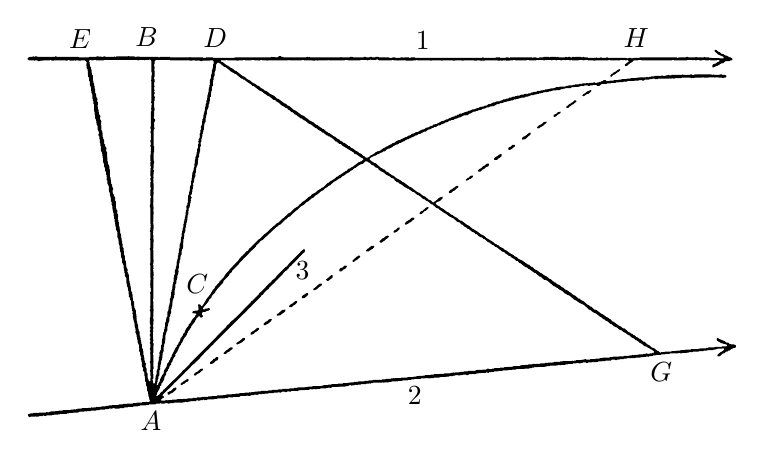
\begin{tikzpicture}[x=0.00600130cm,y=-0.00600130cm]
\fill[even odd rule] (925,359) -- (924,358) -- (921,358) -- (918,361) -- (915,362) -- (912,365) -- (908,367) -- (905,370) -- (905,372) -- (906,373) -- (909,373) -- (911,372) -- (914,369) -- (917,368) -- (922,363) -- (923,363) -- (925,361) -- cycle
(956,337) -- (955,336) -- (951,337) -- (947,341) -- (945,341) -- (941,345) -- (941,346) -- (943,347) -- (947,345) -- (949,343) -- (951,343) -- (956,339) -- cycle
(990,312) -- (989,311) -- (986,311) -- (984,312) -- (981,315) -- (978,316) -- (973,321) -- (970,322) -- (967,325) -- (967,327) -- (968,328) -- (971,328) -- (973,327) -- (977,323) -- (980,322) -- (984,318) -- (988,317) -- (990,314) -- cycle
(1017,292) -- (1016,291) -- (1014,291) -- (1010,293) -- (1008,295) -- (1004,297) -- (1001,300) -- (1001,302) -- (1002,303) -- (1007,303) -- (1011,299) -- (1012,299) -- (1017,295) -- cycle
(1045,272) -- (1044,271) -- (1040,271) -- (1035,276) -- (1033,276) -- (1031,278) -- (1031,281) -- (1032,282) -- (1034,282) -- (1038,280) -- (1045,274) -- cycle
(1078,246) -- (1076,245) -- (1066,253) -- (1063,254) -- (1060,257) -- (1060,259) -- (1061,260) -- (1067,259) -- (1078,249) -- cycle
(1112,222) -- (1106,223) -- (1102,227) -- (1096,230) -- (1092,234) -- (1092,235) -- (1093,236) -- (1096,236) -- (1100,233) -- (1103,232) -- (1112,224) -- cycle
(1142,202) -- (1141,201) -- (1136,202) -- (1132,206) -- (1130,206) -- (1127,209) -- (1127,211) -- (1128,212) -- (1132,211) -- (1136,207) -- (1141,204) -- cycle
(1175,178) -- (1174,177) -- (1171,177) -- (1167,181) -- (1166,181) -- (1164,183) -- (1160,185) -- (1156,189) -- (1155,189) -- (1154,190) -- (1154,192) -- (1155,193) -- (1158,193) -- (1162,189) -- (1163,189) -- (1166,186) -- (1169,185) -- (1173,181) -- (1174,181) -- (1175,180) -- cycle
(1207,156) -- (1206,155) -- (1204,155) -- (1202,157) -- (1198,158) -- (1192,163) -- (1191,163) -- (1188,166) -- (1188,167) -- (1189,168) -- (1191,168) -- (1198,163) -- (1201,163) -- (1207,157) -- cycle
(1268,112) -- (1267,111) -- (1263,112) -- (1257,117) -- (1254,118) -- (1251,121) -- (1250,121) -- (1247,124) -- (1247,126) -- (1249,127) -- (1253,123) -- (1257,122) -- (1260,119) -- (1265,116) -- (1268,113) -- cycle
(1506,89) -- (1502,86) -- (1500,86) -- (1493,82) -- (1491,82) -- (1486,79) -- (1482,78) -- (1479,75) -- (1476,74) -- (1471,70) -- (1469,70) -- (1468,71) -- (1468,73) -- (1477,81) -- (1479,81) -- (1480,82) -- (1482,82) -- (1484,84) -- (1486,84) -- (1487,85) -- (1487,87) -- (1486,88) -- (1457,87) -- (1456,86) -- (1448,86) -- (1447,85) -- (1445,86) -- (1430,86) -- (1429,85) -- (1427,86) -- (1412,86) -- (1411,85) -- (1408,85) -- (1407,86) -- (1392,86) -- (1391,87) -- (1389,87) -- (1388,86) -- (1310,86) -- (1309,87) -- (1295,87) -- (1294,88) -- (1292,88) -- (1291,87) -- (1286,87) -- (1285,88) -- (1282,88) -- (1281,87) -- (1242,87) -- (1241,86) -- (1239,86) -- (1238,87) -- (1229,87) -- (1228,86) -- (1226,86) -- (1225,87) -- (1219,87) -- (1218,86) -- (1216,87) -- (1200,87) -- (1199,86) -- (1192,86) -- (1191,85) -- (1189,85) -- (1188,86) -- (1186,86) -- (1185,85) -- (1173,85) -- (1172,86) -- (1170,85) -- (1167,85) -- (1166,86) -- (1163,86) -- (1162,85) -- (1157,85) -- (1156,86) -- (1154,85) -- (1152,85) -- (1151,86) -- (1138,86) -- (1137,85) -- (1134,85) -- (1133,86) -- (1131,85) -- (1120,85) -- (1118,86) -- (1117,85) -- (1106,85) -- (1105,86) -- (1097,86) -- (1096,87) -- (1091,87) -- (1090,86) -- (1084,86) -- (1083,87) -- (1081,86) -- (1035,86) -- (1034,87) -- (1032,87) -- (1031,86) -- (1026,86) -- (1025,87) -- (1014,87) -- (1013,86) -- (1005,86) -- (1004,87) -- (979,87) -- (978,86) -- (976,86) -- (975,87) -- (834,87) -- (833,86) -- (825,86) -- (824,87) -- (821,87) -- (820,86) -- (811,86) -- (810,87) -- (808,86) -- (803,86) -- (802,87) -- (792,87) -- (791,86) -- (786,86) -- (785,87) -- (779,87) -- (778,86) -- (757,86) -- (756,85) -- (750,85) -- (749,86) -- (743,86) -- (742,85) -- (738,85) -- (737,86) -- (730,86) -- (729,85) -- (725,85) -- (724,86) -- (702,86) -- (701,85) -- (696,85) -- (695,86) -- (678,86) -- (677,85) -- (675,86) -- (611,86) -- (610,85) -- (608,86) -- (606,85) -- (604,85) -- (603,86) -- (555,86) -- (554,85) -- (551,85) -- (549,83) -- (546,83) -- (542,86) -- (529,85) -- (528,86) -- (452,86) -- (451,87) -- (406,87) -- (405,86) -- (391,86) -- (390,87) -- (385,87) -- (384,86) -- (358,86) -- (357,85) -- (355,86) -- (315,86) -- (314,85) -- (293,85) -- (292,86) -- (290,86) -- (289,85) -- (250,85) -- (249,84) -- (240,85) -- (239,84) -- (228,84) -- (227,83) -- (225,84) -- (201,84) -- (200,85) -- (198,85) -- (197,84) -- (195,85) -- (178,85) -- (177,84) -- (174,84) -- (173,85) -- (166,84) -- (164,85) -- (163,84) -- (159,84) -- (158,85) -- (143,85) -- (142,86) -- (122,86) -- (121,85) -- (75,85) -- (74,84) -- (71,84) -- (70,85) -- (34,85) -- (33,84) -- (29,84) -- (27,85) -- (26,84) -- (24,84) -- (23,85) -- (17,85) -- (15,86) -- (13,88) -- (13,90) -- (16,92) -- (26,92) -- (27,93) -- (29,92) -- (33,92) -- (36,94) -- (39,94) -- (40,93) -- (45,93) -- (46,92) -- (60,92) -- (61,91) -- (62,91) -- (64,93) -- (68,93) -- (69,92) -- (93,92) -- (94,93) -- (96,93) -- (100,91) -- (103,93) -- (110,93) -- (111,92) -- (113,92) -- (114,93) -- (116,92) -- (120,92) -- (121,93) -- (125,93) -- (126,92) -- (134,92) -- (138,96) -- (137,103) -- (138,104) -- (138,109) -- (140,111) -- (141,126) -- (143,129) -- (143,135) -- (145,138) -- (145,145) -- (147,149) -- (148,161) -- (150,164) -- (150,173) -- (151,174) -- (151,177) -- (152,178) -- (152,184) -- (154,186) -- (154,200) -- (155,201) -- (155,207) -- (156,208) -- (156,215) -- (158,218) -- (159,227) -- (161,231) -- (161,238) -- (164,244) -- (164,248) -- (163,249) -- (163,251) -- (165,254) -- (165,259) -- (166,260) -- (166,267) -- (167,268) -- (167,273) -- (168,274) -- (168,284) -- (170,286) -- (170,289) -- (171,290) -- (171,294) -- (172,295) -- (172,298) -- (173,299) -- (173,308) -- (175,312) -- (175,317) -- (177,321) -- (177,326) -- (179,329) -- (179,334) -- (180,335) -- (180,339) -- (181,340) -- (180,345) -- (182,347) -- (182,353) -- (185,359) -- (185,369) -- (187,373) -- (187,378) -- (188,379) -- (188,382) -- (189,383) -- (189,389) -- (191,393) -- (191,398) -- (192,399) -- (193,410) -- (194,411) -- (194,414) -- (195,415) -- (195,422) -- (196,423) -- (196,427) -- (197,428) -- (197,434) -- (198,435) -- (198,439) -- (199,440) -- (199,444) -- (200,445) -- (200,450) -- (203,456) -- (203,467) -- (205,470) -- (206,481) -- (208,485) -- (208,491) -- (209,492) -- (209,497) -- (210,498) -- (211,509) -- (213,513) -- (213,520) -- (216,526) -- (216,532) -- (217,533) -- (217,537) -- (218,538) -- (218,542) -- (219,543) -- (219,549) -- (222,553) -- (222,564) -- (223,565) -- (223,570) -- (225,573) -- (225,575) -- (226,576) -- (226,580) -- (227,581) -- (227,588) -- (228,589) -- (227,592) -- (229,594) -- (230,599) -- (232,602) -- (232,611) -- (233,612) -- (233,617) -- (234,618) -- (234,622) -- (236,625) -- (235,627) -- (235,629) -- (236,630) -- (236,638) -- (237,639) -- (237,642) -- (238,643) -- (238,646) -- (239,647) -- (240,658) -- (241,659) -- (241,662) -- (242,663) -- (241,668) -- (244,674) -- (244,678) -- (245,679) -- (245,683) -- (246,684) -- (246,690) -- (249,696) -- (249,702) -- (250,703) -- (249,705) -- (249,708) -- (251,710) -- (251,716) -- (252,717) -- (252,719) -- (254,721) -- (253,723) -- (253,726) -- (254,727) -- (254,730) -- (255,731) -- (255,740) -- (258,745) -- (257,749) -- (260,753) -- (260,760) -- (261,761) -- (261,764) -- (262,765) -- (262,772) -- (264,774) -- (264,781) -- (266,784) -- (266,791) -- (268,795) -- (269,804) -- (270,805) -- (271,811) -- (272,812) -- (272,814) -- (270,816) -- (266,816) -- (264,815) -- (263,816) -- (256,816) -- (255,817) -- (244,817) -- (243,818) -- (237,818) -- (236,819) -- (224,819) -- (223,820) -- (215,820) -- (214,821) -- (207,821) -- (206,822) -- (185,823) -- (184,824) -- (179,824) -- (178,825) -- (170,825) -- (169,826) -- (163,826) -- (162,827) -- (159,826) -- (158,827) -- (153,827) -- (152,828) -- (148,827) -- (147,828) -- (141,828) -- (140,829) -- (128,829) -- (127,830) -- (119,830) -- (118,831) -- (115,831) -- (114,832) -- (111,831) -- (110,832) -- (104,832) -- (103,833) -- (88,833) -- (87,834) -- (79,834) -- (78,835) -- (61,836) -- (57,838) -- (53,837) -- (52,838) -- (25,839) -- (24,840) -- (19,840) -- (18,841) -- (15,841) -- (14,842) -- (14,845) -- (16,848) -- (18,848) -- (19,847) -- (28,847) -- (29,846) -- (31,847) -- (35,847) -- (39,845) -- (43,846) -- (46,844) -- (48,845) -- (52,845) -- (53,844) -- (64,844) -- (65,843) -- (81,842) -- (82,841) -- (95,841) -- (96,840) -- (100,840) -- (101,839) -- (120,838) -- (123,836) -- (133,836) -- (134,835) -- (138,836) -- (139,835) -- (146,835) -- (147,834) -- (158,834) -- (159,833) -- (165,833) -- (166,832) -- (176,832) -- (177,831) -- (183,831) -- (187,829) -- (189,830) -- (192,830) -- (193,829) -- (197,829) -- (198,830) -- (207,830) -- (208,829) -- (216,829) -- (218,827) -- (225,827) -- (226,826) -- (236,826) -- (237,825) -- (246,825) -- (247,824) -- (250,824) -- (251,823) -- (263,823) -- (264,822) -- (269,822) -- (270,821) -- (283,821) -- (286,819) -- (293,819) -- (294,818) -- (296,819) -- (303,819) -- (304,818) -- (309,818) -- (310,819) -- (313,819) -- (314,818) -- (322,818) -- (323,817) -- (342,817) -- (343,816) -- (346,816) -- (347,815) -- (352,816) -- (353,815) -- (357,815) -- (358,814) -- (369,814) -- (371,812) -- (373,812) -- (374,813) -- (378,813) -- (379,812) -- (383,812) -- (384,811) -- (386,811) -- (387,812) -- (390,811) -- (392,812) -- (394,810) -- (408,810) -- (409,809) -- (414,809) -- (415,808) -- (430,808) -- (431,807) -- (436,807) -- (440,805) -- (442,806) -- (448,806) -- (449,805) -- (461,805) -- (464,803) -- (476,803) -- (477,802) -- (483,803) -- (487,801) -- (492,801) -- (493,800) -- (497,800) -- (499,801) -- (503,799) -- (510,799) -- (511,798) -- (514,799) -- (515,798) -- (522,798) -- (523,797) -- (533,797) -- (534,796) -- (542,796) -- (543,795) -- (549,796) -- (552,794) -- (557,794) -- (558,795) -- (560,795) -- (564,793) -- (570,794) -- (572,792) -- (583,792) -- (585,793) -- (587,791) -- (609,790) -- (611,788) -- (613,789) -- (618,789) -- (619,788) -- (624,789) -- (625,788) -- (632,788) -- (633,787) -- (645,787) -- (646,786) -- (649,786) -- (650,785) -- (655,786) -- (658,784) -- (669,784) -- (670,783) -- (672,784) -- (674,783) -- (686,783) -- (687,782) -- (691,782) -- (695,780) -- (697,780) -- (698,781) -- (706,780) -- (707,779) -- (711,780) -- (712,779) -- (718,779) -- (719,778) -- (729,778) -- (730,777) -- (735,777) -- (736,776) -- (739,777) -- (740,776) -- (743,776) -- (744,775) -- (763,775) -- (764,774) -- (768,775) -- (769,774) -- (778,774) -- (779,773) -- (783,773) -- (784,772) -- (797,772) -- (798,771) -- (806,771) -- (807,770) -- (818,770) -- (819,769) -- (825,769) -- (826,768) -- (831,768) -- (832,767) -- (845,767) -- (846,766) -- (855,766) -- (856,765) -- (861,765) -- (862,766) -- (865,766) -- (866,765) -- (873,765) -- (874,764) -- (885,764) -- (886,763) -- (905,762) -- (906,761) -- (914,761) -- (915,760) -- (918,760) -- (919,759) -- (925,759) -- (926,760) -- (928,759) -- (934,759) -- (935,758) -- (942,758) -- (943,759) -- (945,759) -- (948,757) -- (954,757) -- (955,756) -- (961,757) -- (964,755) -- (968,755) -- (969,754) -- (971,755) -- (973,754) -- (983,754) -- (984,753) -- (989,754) -- (991,752) -- (994,753) -- (995,752) -- (1000,752) -- (1001,751) -- (1009,751) -- (1010,750) -- (1018,750) -- (1019,749) -- (1030,749) -- (1031,748) -- (1047,747) -- (1048,746) -- (1075,745) -- (1076,744) -- (1080,744) -- (1081,743) -- (1085,743) -- (1086,742) -- (1111,741) -- (1112,740) -- (1118,740) -- (1119,739) -- (1132,739) -- (1133,738) -- (1136,738) -- (1137,737) -- (1142,738) -- (1143,737) -- (1151,737) -- (1152,736) -- (1157,736) -- (1158,735) -- (1167,735) -- (1168,734) -- (1175,734) -- (1176,733) -- (1179,733) -- (1180,734) -- (1184,734) -- (1185,733) -- (1188,733) -- (1189,732) -- (1195,732) -- (1196,733) -- (1199,733) -- (1200,732) -- (1220,731) -- (1221,730) -- (1228,730) -- (1229,729) -- (1236,729) -- (1237,728) -- (1248,728) -- (1250,726) -- (1257,726) -- (1258,727) -- (1260,727) -- (1261,726) -- (1266,726) -- (1267,725) -- (1275,725) -- (1276,724) -- (1281,724) -- (1282,723) -- (1299,723) -- (1300,722) -- (1310,722) -- (1311,721) -- (1317,721) -- (1318,720) -- (1323,720) -- (1324,719) -- (1328,720) -- (1329,719) -- (1337,718) -- (1338,717) -- (1343,717) -- (1344,716) -- (1354,716) -- (1355,715) -- (1363,715) -- (1364,714) -- (1372,714) -- (1373,713) -- (1390,713) -- (1391,712) -- (1395,712) -- (1396,713) -- (1398,713) -- (1399,712) -- (1408,712) -- (1409,711) -- (1413,711) -- (1414,710) -- (1421,710) -- (1422,709) -- (1434,709) -- (1435,708) -- (1444,708) -- (1445,707) -- (1452,707) -- (1453,706) -- (1464,706) -- (1465,705) -- (1469,705) -- (1470,704) -- (1473,704) -- (1474,703) -- (1484,703) -- (1485,702) -- (1487,702) -- (1488,703) -- (1488,705) -- (1485,708) -- (1478,712) -- (1474,716) -- (1474,718) -- (1475,719) -- (1478,719) -- (1480,718) -- (1485,713) -- (1488,713) -- (1492,709) -- (1495,709) -- (1497,707) -- (1499,707) -- (1503,704) -- (1509,701) -- (1511,701) -- (1513,699) -- (1513,696) -- (1509,694) -- (1503,694) -- (1502,693) -- (1500,693) -- (1498,691) -- (1496,690) -- (1493,690) -- (1489,687) -- (1477,682) -- (1475,680) -- (1474,680) -- (1472,682) -- (1473,686) -- (1482,691) -- (1493,694) -- (1495,696) -- (1493,698) -- (1484,698) -- (1483,699) -- (1469,699) -- (1468,700) -- (1455,700) -- (1454,701) -- (1451,701) -- (1450,702) -- (1438,702) -- (1437,703) -- (1434,703) -- (1433,704) -- (1418,704) -- (1417,705) -- (1406,705) -- (1405,706) -- (1396,706) -- (1395,707) -- (1390,707) -- (1389,708) -- (1386,707) -- (1385,708) -- (1377,708) -- (1376,709) -- (1363,709) -- (1362,710) -- (1355,710) -- (1354,711) -- (1352,711) -- (1349,708) -- (1346,707) -- (1340,702) -- (1334,700) -- (1330,696) -- (1326,694) -- (1319,688) -- (1317,688) -- (1310,682) -- (1308,682) -- (1305,679) -- (1303,679) -- (1299,675) -- (1296,674) -- (1293,671) -- (1291,671) -- (1289,669) -- (1285,667) -- (1277,660) -- (1274,660) -- (1268,655) -- (1265,654) -- (1254,646) -- (1251,645) -- (1248,641) -- (1247,641) -- (1242,637) -- (1239,636) -- (1231,630) -- (1228,629) -- (1219,622) -- (1215,620) -- (1213,620) -- (1207,614) -- (1205,614) -- (1202,611) -- (1199,610) -- (1191,603) -- (1185,600) -- (1182,597) -- (1180,597) -- (1173,591) -- (1167,588) -- (1163,584) -- (1162,584) -- (1157,580) -- (1152,578) -- (1148,574) -- (1145,573) -- (1139,568) -- (1134,566) -- (1131,563) -- (1128,562) -- (1121,556) -- (1118,555) -- (1112,550) -- (1106,547) -- (1103,544) -- (1100,543) -- (1092,537) -- (1087,535) -- (1082,530) -- (1079,529) -- (1075,525) -- (1073,525) -- (1060,516) -- (1053,513) -- (1049,509) -- (1044,507) -- (1041,504) -- (1035,501) -- (1027,495) -- (1024,494) -- (1021,491) -- (1013,487) -- (1010,484) -- (1007,483) -- (1005,481) -- (1003,481) -- (999,477) -- (984,468) -- (980,464) -- (972,460) -- (966,455) -- (954,448) -- (947,442) -- (944,441) -- (932,432) -- (928,431) -- (921,425) -- (918,424) -- (913,420) -- (910,419) -- (904,414) -- (901,413) -- (892,406) -- (889,405) -- (886,402) -- (880,399) -- (877,396) -- (877,395) -- (880,392) -- (886,390) -- (892,384) -- (892,382) -- (891,381) -- (885,383) -- (876,391) -- (875,391) -- (873,393) -- (871,393) -- (867,389) -- (862,387) -- (855,381) -- (854,381) -- (852,379) -- (850,379) -- (843,373) -- (838,371) -- (825,361) -- (822,360) -- (810,351) -- (807,350) -- (802,346) -- (794,342) -- (787,336) -- (785,336) -- (782,333) -- (781,333) -- (776,329) -- (773,328) -- (768,323) -- (766,323) -- (764,321) -- (760,319) -- (750,310) -- (748,310) -- (740,305) -- (737,302) -- (737,301) -- (740,298) -- (748,294) -- (750,294) -- (755,290) -- (756,291) -- (760,288) -- (764,287) -- (766,285) -- (769,285) -- (773,281) -- (777,279) -- (779,279) -- (785,276) -- (787,274) -- (795,270) -- (797,270) -- (801,267) -- (803,267) -- (808,264) -- (810,264) -- (812,262) -- (818,259) -- (820,259) -- (822,257) -- (824,257) -- (826,255) -- (828,255) -- (835,251) -- (837,251) -- (841,248) -- (844,248) -- (853,243) -- (856,243) -- (861,239) -- (866,238) -- (870,235) -- (872,235) -- (874,233) -- (878,233) -- (882,230) -- (886,230) -- (890,227) -- (892,227) -- (893,226) -- (895,226) -- (897,224) -- (902,223) -- (906,220) -- (909,220) -- (911,218) -- (915,218) -- (918,216) -- (923,215) -- (926,213) -- (929,213) -- (936,209) -- (945,208) -- (948,205) -- (950,205) -- (957,201) -- (961,201) -- (963,199) -- (966,199) -- (970,197) -- (974,197) -- (976,195) -- (982,194) -- (985,192) -- (989,192) -- (992,190) -- (1000,189) -- (1007,185) -- (1011,185) -- (1013,183) -- (1017,183) -- (1024,180) -- (1027,180) -- (1028,179) -- (1031,179) -- (1032,178) -- (1035,178) -- (1036,177) -- (1040,177) -- (1043,175) -- (1047,175) -- (1048,174) -- (1054,173) -- (1055,172) -- (1058,172) -- (1059,171) -- (1065,171) -- (1068,169) -- (1072,169) -- (1079,166) -- (1084,166) -- (1085,165) -- (1091,164) -- (1092,163) -- (1095,163) -- (1096,162) -- (1100,162) -- (1101,161) -- (1104,161) -- (1105,160) -- (1116,159) -- (1117,158) -- (1120,158) -- (1121,157) -- (1124,157) -- (1125,156) -- (1140,155) -- (1143,153) -- (1147,153) -- (1148,152) -- (1151,152) -- (1152,151) -- (1163,151) -- (1165,149) -- (1181,148) -- (1185,146) -- (1188,146) -- (1190,147) -- (1193,145) -- (1199,145) -- (1200,146) -- (1203,146) -- (1204,145) -- (1210,145) -- (1211,144) -- (1217,144) -- (1219,146) -- (1224,146) -- (1229,142) -- (1239,142) -- (1240,141) -- (1248,141) -- (1249,140) -- (1258,140) -- (1259,139) -- (1274,138) -- (1275,137) -- (1282,137) -- (1283,136) -- (1307,135) -- (1308,134) -- (1314,134) -- (1315,135) -- (1318,135) -- (1320,133) -- (1329,133) -- (1330,132) -- (1335,132) -- (1336,131) -- (1341,131) -- (1342,132) -- (1347,132) -- (1348,131) -- (1371,131) -- (1372,130) -- (1374,131) -- (1376,131) -- (1377,130) -- (1383,131) -- (1384,130) -- (1397,130) -- (1398,129) -- (1417,129) -- (1418,130) -- (1422,129) -- (1424,130) -- (1425,129) -- (1441,129) -- (1442,128) -- (1444,128) -- (1445,129) -- (1454,129) -- (1455,128) -- (1467,128) -- (1469,129) -- (1470,128) -- (1476,128) -- (1477,129) -- (1484,129) -- (1486,130) -- (1487,129) -- (1490,129) -- (1493,127) -- (1493,125) -- (1490,123) -- (1484,123) -- (1483,122) -- (1479,122) -- (1478,123) -- (1467,123) -- (1466,122) -- (1464,123) -- (1462,123) -- (1461,122) -- (1426,122) -- (1425,123) -- (1420,123) -- (1419,122) -- (1417,122) -- (1416,123) -- (1402,123) -- (1400,122) -- (1399,123) -- (1377,123) -- (1376,124) -- (1372,124) -- (1371,123) -- (1369,123) -- (1368,124) -- (1365,124) -- (1364,125) -- (1358,125) -- (1357,124) -- (1355,125) -- (1341,125) -- (1340,126) -- (1334,126) -- (1333,127) -- (1329,127) -- (1328,128) -- (1326,128) -- (1325,127) -- (1323,128) -- (1309,128) -- (1308,129) -- (1303,129) -- (1302,130) -- (1290,130) -- (1289,131) -- (1282,131) -- (1281,132) -- (1271,132) -- (1270,133) -- (1265,133) -- (1264,134) -- (1255,134) -- (1254,135) -- (1246,135) -- (1245,136) -- (1239,136) -- (1237,134) -- (1233,134) -- (1231,136) -- (1229,136) -- (1227,138) -- (1224,138) -- (1223,139) -- (1220,139) -- (1219,140) -- (1215,140) -- (1214,139) -- (1211,139) -- (1210,140) -- (1203,140) -- (1202,141) -- (1197,140) -- (1196,141) -- (1188,141) -- (1187,142) -- (1181,142) -- (1180,143) -- (1173,143) -- (1172,144) -- (1168,144) -- (1167,145) -- (1159,145) -- (1158,146) -- (1155,146) -- (1151,148) -- (1140,148) -- (1139,149) -- (1132,149) -- (1130,151) -- (1119,152) -- (1118,153) -- (1109,154) -- (1108,155) -- (1100,156) -- (1099,157) -- (1093,157) -- (1090,159) -- (1085,159) -- (1084,160) -- (1081,160) -- (1078,162) -- (1074,162) -- (1073,163) -- (1066,163) -- (1063,165) -- (1058,165) -- (1054,167) -- (1050,167) -- (1049,168) -- (1046,168) -- (1045,169) -- (1041,169) -- (1037,171) -- (1033,171) -- (1031,173) -- (1028,173) -- (1024,175) -- (1020,175) -- (1018,177) -- (1016,177) -- (1012,179) -- (1006,179) -- (1003,181) -- (1000,181) -- (992,185) -- (989,185) -- (985,188) -- (982,188) -- (978,190) -- (971,191) -- (969,193) -- (966,193) -- (959,196) -- (955,196) -- (952,198) -- (947,199) -- (944,201) -- (942,201) -- (941,202) -- (939,202) -- (932,205) -- (929,205) -- (926,207) -- (924,207) -- (922,209) -- (919,209) -- (917,211) -- (912,212) -- (909,214) -- (907,214) -- (903,217) -- (900,217) -- (895,220) -- (890,221) -- (879,227) -- (873,228) -- (870,231) -- (867,231) -- (862,234) -- (857,235) -- (853,238) -- (848,239) -- (839,244) -- (836,244) -- (831,247) -- (827,248) -- (823,251) -- (819,252) -- (815,255) -- (813,255) -- (801,261) -- (799,261) -- (793,264) -- (791,266) -- (785,268) -- (783,270) -- (778,272) -- (776,274) -- (772,275) -- (770,277) -- (767,278) -- (760,283) -- (756,285) -- (755,284) -- (753,286) -- (751,286) -- (747,290) -- (745,290) -- (742,293) -- (740,293) -- (736,297) -- (734,298) -- (729,298) -- (727,296) -- (723,294) -- (719,290) -- (716,289) -- (711,285) -- (708,284) -- (702,279) -- (699,278) -- (695,274) -- (693,274) -- (684,267) -- (682,267) -- (679,264) -- (676,263) -- (673,260) -- (670,259) -- (664,254) -- (661,253) -- (653,247) -- (650,246) -- (648,244) -- (644,242) -- (640,238) -- (638,238) -- (635,235) -- (634,235) -- (626,229) -- (623,228) -- (619,224) -- (609,219) -- (605,215) -- (604,215) -- (598,210) -- (593,208) -- (581,199) -- (576,197) -- (575,195) -- (574,195) -- (567,189) -- (564,188) -- (560,184) -- (558,184) -- (544,174) -- (541,173) -- (536,168) -- (526,163) -- (520,158) -- (515,156) -- (513,154) -- (506,150) -- (502,146) -- (500,146) -- (495,142) -- (490,140) -- (484,135) -- (478,132) -- (471,126) -- (469,126) -- (455,115) -- (452,114) -- (446,109) -- (443,108) -- (438,104) -- (435,103) -- (426,96) -- (424,96) -- (422,94) -- (422,93) -- (424,91) -- (426,92) -- (432,92) -- (433,91) -- (435,91) -- (436,92) -- (455,92) -- (456,93) -- (459,93) -- (460,92) -- (469,92) -- (470,91) -- (472,91) -- (473,92) -- (487,92) -- (488,91) -- (492,91) -- (493,92) -- (502,92) -- (503,93) -- (507,91) -- (509,91) -- (510,92) -- (519,92) -- (520,93) -- (522,92) -- (565,92) -- (566,91) -- (568,92) -- (593,92) -- (594,91) -- (597,91) -- (598,92) -- (616,92) -- (617,93) -- (625,92) -- (627,93) -- (628,92) -- (648,92) -- (649,91) -- (651,92) -- (684,92) -- (685,91) -- (690,91) -- (691,92) -- (717,92) -- (718,91) -- (731,91) -- (732,92) -- (734,92) -- (735,91) -- (738,91) -- (739,90) -- (741,91) -- (751,91) -- (752,90) -- (754,90) -- (757,92) -- (784,92) -- (785,91) -- (787,91) -- (788,92) -- (796,92) -- (797,93) -- (799,92) -- (829,93) -- (830,92) -- (835,92) -- (836,91) -- (838,92) -- (865,92) -- (866,93) -- (868,93) -- (869,92) -- (888,92) -- (889,93) -- (891,93) -- (892,92) -- (913,92) -- (914,93) -- (918,93) -- (919,92) -- (932,92) -- (933,93) -- (936,93) -- (937,92) -- (958,92) -- (959,93) -- (964,93) -- (965,92) -- (970,92) -- (971,93) -- (981,93) -- (982,92) -- (1008,92) -- (1009,93) -- (1013,93) -- (1015,92) -- (1016,93) -- (1019,93) -- (1020,92) -- (1026,92) -- (1027,93) -- (1033,93) -- (1034,92) -- (1041,92) -- (1042,91) -- (1045,91) -- (1046,92) -- (1070,92) -- (1071,91) -- (1074,91) -- (1075,92) -- (1090,92) -- (1091,91) -- (1093,91) -- (1094,92) -- (1096,91) -- (1101,91) -- (1102,92) -- (1104,91) -- (1106,92) -- (1108,92) -- (1109,91) -- (1111,92) -- (1113,91) -- (1121,91) -- (1122,92) -- (1124,92) -- (1125,91) -- (1131,91) -- (1132,92) -- (1134,92) -- (1135,91) -- (1141,91) -- (1142,92) -- (1145,92) -- (1146,91) -- (1151,91) -- (1152,92) -- (1154,91) -- (1160,91) -- (1161,92) -- (1163,92) -- (1164,91) -- (1166,92) -- (1180,92) -- (1181,91) -- (1188,91) -- (1189,92) -- (1192,92) -- (1193,91) -- (1199,91) -- (1200,92) -- (1211,92) -- (1212,93) -- (1215,93) -- (1216,92) -- (1243,92) -- (1244,91) -- (1246,91) -- (1247,92) -- (1268,92) -- (1269,91) -- (1272,91) -- (1273,92) -- (1278,91) -- (1279,92) -- (1281,92) -- (1283,91) -- (1287,94) -- (1278,101) -- (1278,103) -- (1279,104) -- (1282,104) -- (1289,98) -- (1293,96) -- (1297,92) -- (1306,92) -- (1307,91) -- (1312,91) -- (1313,92) -- (1378,92) -- (1379,91) -- (1381,91) -- (1382,92) -- (1409,92) -- (1410,91) -- (1420,91) -- (1421,92) -- (1426,91) -- (1427,92) -- (1430,92) -- (1431,91) -- (1435,91) -- (1437,93) -- (1439,92) -- (1442,92) -- (1443,91) -- (1447,91) -- (1448,92) -- (1456,92) -- (1457,91) -- (1459,92) -- (1472,92) -- (1473,91) -- (1477,91) -- (1478,92) -- (1478,94) -- (1477,95) -- (1474,96) -- (1470,99) -- (1466,100) -- (1463,103) -- (1463,106) -- (1464,107) -- (1466,107) -- (1467,106) -- (1469,106) -- (1471,104) -- (1473,104) -- (1477,102) -- (1481,99) -- (1486,98) -- (1491,94) -- (1499,94) -- (1502,92) -- (1504,92) -- (1506,90) -- cycle
(285,802) -- (287,799) -- (287,796) -- (289,794) -- (289,792) -- (291,790) -- (293,786) -- (293,783) -- (296,780) -- (296,777) -- (298,775) -- (302,768) -- (303,762) -- (306,758) -- (306,754) -- (310,749) -- (310,747) -- (312,745) -- (314,739) -- (317,736) -- (317,733) -- (320,729) -- (320,727) -- (323,721) -- (326,718) -- (326,714) -- (330,709) -- (335,697) -- (338,694) -- (338,692) -- (340,690) -- (344,681) -- (349,675) -- (353,666) -- (356,663) -- (356,661) -- (359,658) -- (359,656) -- (367,646) -- (368,643) -- (370,641) -- (370,639) -- (375,634) -- (377,634) -- (379,636) -- (379,637) -- (381,637) -- (384,635) -- (384,633) -- (382,631) -- (382,627) -- (384,625) -- (389,625) -- (392,623) -- (397,622) -- (399,620) -- (399,619) -- (397,617) -- (395,617) -- (394,618) -- (389,618) -- (387,620) -- (386,620) -- (384,618) -- (384,617) -- (395,604) -- (398,598) -- (402,595) -- (403,591) -- (410,584) -- (411,581) -- (414,578) -- (414,577) -- (427,563) -- (428,559) -- (439,548) -- (441,544) -- (445,541) -- (446,538) -- (461,523) -- (461,522) -- (470,513) -- (470,512) -- (472,510) -- (473,510) -- (481,502) -- (481,501) -- (496,487) -- (497,484) -- (499,482) -- (500,482) -- (507,474) -- (510,473) -- (540,445) -- (541,445) -- (545,441) -- (548,440) -- (559,429) -- (560,429) -- (565,424) -- (568,423) -- (577,414) -- (578,414) -- (582,410) -- (583,410) -- (591,402) -- (598,398) -- (604,392) -- (607,391) -- (615,384) -- (618,383) -- (623,378) -- (628,375) -- (636,368) -- (638,368) -- (643,363) -- (647,361) -- (650,358) -- (653,357) -- (662,349) -- (665,348) -- (673,342) -- (675,342) -- (679,338) -- (685,335) -- (688,332) -- (694,329) -- (697,326) -- (700,325) -- (704,321) -- (707,320) -- (715,314) -- (719,312) -- (722,312) -- (728,306) -- (732,306) -- (734,308) -- (737,309) -- (742,314) -- (746,315) -- (750,319) -- (754,320) -- (756,322) -- (756,323) -- (761,327) -- (766,329) -- (772,334) -- (780,338) -- (783,341) -- (787,342) -- (790,345) -- (790,346) -- (795,350) -- (797,350) -- (800,353) -- (806,356) -- (812,361) -- (815,362) -- (817,364) -- (819,364) -- (829,371) -- (831,371) -- (838,377) -- (840,377) -- (842,379) -- (843,379) -- (851,386) -- (853,386) -- (858,390) -- (861,391) -- (868,397) -- (870,397) -- (879,405) -- (883,406) -- (887,410) -- (888,410) -- (896,416) -- (899,417) -- (905,422) -- (915,427) -- (924,435) -- (927,435) -- (932,440) -- (934,440) -- (938,444) -- (942,446) -- (945,449) -- (947,449) -- (954,455) -- (959,457) -- (962,460) -- (964,460) -- (969,465) -- (973,467) -- (975,467) -- (979,471) -- (981,471) -- (988,477) -- (991,478) -- (997,483) -- (999,483) -- (1003,487) -- (1005,487) -- (1018,497) -- (1022,498) -- (1026,502) -- (1027,502) -- (1032,506) -- (1035,507) -- (1038,510) -- (1044,513) -- (1048,517) -- (1051,517) -- (1054,521) -- (1057,522) -- (1067,530) -- (1071,531) -- (1074,534) -- (1075,534) -- (1086,542) -- (1089,543) -- (1097,550) -- (1099,550) -- (1107,557) -- (1110,557) -- (1114,559) -- (1128,571) -- (1130,571) -- (1132,573) -- (1135,574) -- (1138,577) -- (1146,581) -- (1151,586) -- (1154,587) -- (1156,589) -- (1160,590) -- (1172,600) -- (1175,601) -- (1182,606) -- (1191,610) -- (1202,620) -- (1205,621) -- (1211,626) -- (1218,629) -- (1225,635) -- (1228,636) -- (1232,640) -- (1235,641) -- (1238,644) -- (1240,644) -- (1247,650) -- (1250,651) -- (1254,655) -- (1261,658) -- (1267,663) -- (1271,664) -- (1274,667) -- (1280,670) -- (1285,674) -- (1287,674) -- (1292,679) -- (1297,681) -- (1301,685) -- (1303,685) -- (1305,687) -- (1306,687) -- (1310,691) -- (1313,692) -- (1320,698) -- (1323,698) -- (1327,701) -- (1329,701) -- (1332,704) -- (1335,705) -- (1340,709) -- (1340,710) -- (1338,712) -- (1336,712) -- (1335,713) -- (1331,713) -- (1330,714) -- (1326,714) -- (1325,713) -- (1323,713) -- (1322,714) -- (1317,714) -- (1316,715) -- (1307,715) -- (1306,716) -- (1298,716) -- (1297,717) -- (1294,716) -- (1293,717) -- (1288,717) -- (1287,718) -- (1276,718) -- (1275,719) -- (1252,720) -- (1251,721) -- (1246,721) -- (1245,722) -- (1231,722) -- (1230,723) -- (1225,723) -- (1224,724) -- (1216,724) -- (1215,725) -- (1205,725) -- (1204,726) -- (1196,726) -- (1195,725) -- (1193,725) -- (1192,726) -- (1187,726) -- (1186,727) -- (1175,727) -- (1174,728) -- (1171,728) -- (1170,729) -- (1168,729) -- (1167,728) -- (1165,729) -- (1147,729) -- (1146,730) -- (1141,730) -- (1140,731) -- (1128,731) -- (1127,732) -- (1109,733) -- (1108,734) -- (1099,734) -- (1098,735) -- (1090,735) -- (1089,736) -- (1087,735) -- (1083,735) -- (1082,736) -- (1074,736) -- (1073,737) -- (1058,738) -- (1054,740) -- (1042,740) -- (1041,741) -- (1023,742) -- (1022,743) -- (1014,743) -- (1013,744) -- (1002,744) -- (1001,745) -- (997,745) -- (996,746) -- (990,746) -- (989,745) -- (987,745) -- (984,747) -- (977,747) -- (976,748) -- (964,748) -- (960,750) -- (946,750) -- (945,751) -- (937,751) -- (936,752) -- (928,752) -- (927,753) -- (919,753) -- (918,754) -- (914,753) -- (913,754) -- (909,754) -- (908,755) -- (896,755) -- (895,756) -- (887,756) -- (886,757) -- (874,757) -- (873,758) -- (867,758) -- (866,759) -- (855,759) -- (854,760) -- (837,761) -- (836,762) -- (831,762) -- (830,763) -- (818,763) -- (817,764) -- (805,764) -- (804,765) -- (792,765) -- (791,766) -- (788,765) -- (787,766) -- (783,766) -- (782,767) -- (771,767) -- (770,768) -- (764,768) -- (763,769) -- (745,769) -- (744,770) -- (736,770) -- (735,771) -- (727,771) -- (726,772) -- (714,772) -- (713,773) -- (705,773) -- (704,774) -- (698,774) -- (697,775) -- (692,775) -- (691,776) -- (681,776) -- (680,777) -- (670,777) -- (669,778) -- (657,778) -- (656,779) -- (650,779) -- (649,780) -- (640,780) -- (639,781) -- (636,781) -- (635,782) -- (617,782) -- (616,783) -- (608,783) -- (607,784) -- (604,784) -- (603,785) -- (601,784) -- (599,785) -- (585,785) -- (584,786) -- (578,786) -- (577,787) -- (568,787) -- (567,788) -- (553,788) -- (552,789) -- (544,789) -- (543,790) -- (531,790) -- (530,791) -- (523,791) -- (522,792) -- (508,792) -- (507,793) -- (494,794) -- (493,795) -- (487,795) -- (486,796) -- (483,795) -- (482,796) -- (473,796) -- (472,797) -- (462,797) -- (461,798) -- (454,798) -- (453,799) -- (433,800) -- (432,801) -- (427,801) -- (426,802) -- (415,802) -- (414,803) -- (396,804) -- (395,805) -- (382,805) -- (381,806) -- (372,806) -- (371,807) -- (363,807) -- (362,808) -- (352,808) -- (351,809) -- (329,810) -- (328,811) -- (319,811) -- (318,812) -- (311,812) -- (310,813) -- (309,812) -- (305,812) -- (304,813) -- (296,813) -- (295,811) -- (298,808) -- (302,806) -- (302,805) -- (298,801) -- (311,788) -- (312,788) -- (322,778) -- (322,777) -- (325,774) -- (326,774) -- (346,754) -- (346,753) -- (348,751) -- (349,751) -- (359,741) -- (359,740) -- (363,736) -- (364,736) -- (379,722) -- (379,721) -- (386,714) -- (386,713) -- (393,706) -- (394,706) -- (399,701) -- (399,700) -- (403,696) -- (404,696) -- (407,693) -- (407,692) -- (462,637) -- (463,637) -- (463,636) -- (471,628) -- (472,628) -- (484,615) -- (485,615) -- (487,613) -- (487,612) -- (507,592) -- (507,591) -- (509,589) -- (510,589) -- (513,586) -- (513,585) -- (520,578) -- (521,578) -- (524,575) -- (524,574) -- (533,565) -- (534,565) -- (540,558) -- (542,557) -- (542,556) -- (554,544) -- (554,543) -- (559,538) -- (560,538) -- (566,532) -- (566,531) -- (569,528) -- (570,528) -- (597,500) -- (599,499) -- (600,497) -- (600,493) -- (598,492) -- (593,496) -- (592,496) -- (591,498) -- (565,524) -- (565,525) -- (560,530) -- (559,530) -- (540,549) -- (540,550) -- (534,556) -- (533,556) -- (529,560) -- (529,561) -- (527,563) -- (526,563) -- (507,583) -- (506,583) -- (503,586) -- (503,587) -- (488,602) -- (486,603) -- (486,604) -- (470,620) -- (470,621) -- (468,623) -- (467,623) -- (466,625) -- (453,638) -- (452,638) -- (447,643) -- (446,643) -- (442,647) -- (442,648) -- (434,655) -- (434,656) -- (413,677) -- (413,678) -- (356,735) -- (356,736) -- (344,748) -- (343,748) -- (340,751) -- (340,752) -- (300,791) -- (300,792) -- (298,794) -- (297,794) -- (293,798) -- (293,799) -- (291,801) -- (290,801) -- (287,804) -- cycle
(328,786) -- (327,785) -- (323,786) -- (316,793) -- (314,793) -- (309,796) -- (310,800) -- (313,800) -- (317,797) -- (320,796) -- (328,789) -- cycle
(354,769) -- (352,767) -- (349,768) -- (347,770) -- (344,771) -- (341,774) -- (340,774) -- (337,777) -- (337,779) -- (338,780) -- (340,780) -- (342,778) -- (345,777) -- (348,774) -- (351,773) -- (354,770) -- cycle
(384,746) -- (383,745) -- (379,746) -- (372,752) -- (369,753) -- (365,757) -- (365,758) -- (367,760) -- (368,760) -- (373,756) -- (376,755) -- (384,748) -- cycle
(417,722) -- (416,721) -- (412,721) -- (409,724) -- (406,725) -- (405,727) -- (399,732) -- (399,734) -- (400,735) -- (403,735) -- (407,733) -- (412,728) -- (414,728) -- (416,726) -- cycle
(447,701) -- (446,700) -- (443,700) -- (441,701) -- (435,706) -- (434,706) -- (428,712) -- (428,713) -- (429,714) -- (432,714) -- (434,713) -- (437,710) -- (440,709) -- (444,705) -- (445,705) -- (447,703) -- cycle
(473,681) -- (472,680) -- (468,681) -- (464,685) -- (455,691) -- (455,693) -- (457,694) -- (466,690) -- (473,684) -- cycle
(503,660) -- (502,659) -- (499,659) -- (492,665) -- (488,667) -- (485,670) -- (485,672) -- (486,673) -- (488,673) -- (492,671) -- (495,668) -- (499,666) -- (503,662) -- cycle
(530,641) -- (529,640) -- (526,640) -- (524,641) -- (521,644) -- (517,646) -- (513,650) -- (513,652) -- (514,653) -- (517,653) -- (519,651) -- (522,650) -- (528,645) -- cycle
(559,621) -- (558,620) -- (552,621) -- (543,629) -- (542,629) -- (541,630) -- (541,632) -- (542,633) -- (548,632) -- (554,627) -- (555,627) -- (559,623) -- cycle
(584,603) -- (583,602) -- (580,602) -- (574,607) -- (570,609) -- (567,612) -- (567,614) -- (568,615) -- (571,615) -- (573,614) -- (576,611) -- (579,610) -- (583,606) -- cycle
(607,586) -- (606,585) -- (604,585) -- (596,590) -- (594,592) -- (594,595) -- (595,596) -- (598,596) -- (600,595) -- (607,589) -- cycle
(636,566) -- (635,565) -- (632,565) -- (630,566) -- (620,575) -- (619,575) -- (618,576) -- (618,578) -- (619,579) -- (621,579) -- (625,577) -- (632,571) -- (633,571) -- (636,568) -- cycle
(659,548) -- (658,547) -- (656,547) -- (647,555) -- (646,555) -- (645,557) -- (647,559) -- (650,559) -- (659,552) -- cycle
(689,528) -- (688,527) -- (684,527) -- (680,531) -- (676,532) -- (673,535) -- (673,538) -- (674,539) -- (677,539) -- (679,538) -- (682,535) -- (685,534) -- (688,531) -- cycle
(717,507) -- (716,506) -- (713,506) -- (711,508) -- (710,508) -- (701,516) -- (701,518) -- (702,519) -- (704,519) -- (706,517) -- (710,515) -- (717,509) -- cycle
(747,486) -- (746,485) -- (742,485) -- (740,486) -- (734,491) -- (733,491) -- (730,494) -- (730,496) -- (731,497) -- (735,497) -- (738,494) -- (740,494) -- (742,492) -- (743,492) -- (746,489) -- cycle
(778,465) -- (776,463) -- (771,465) -- (768,468) -- (765,469) -- (760,474) -- (759,474) -- (758,476) -- (760,478) -- (763,478) -- (765,476) -- (768,475) -- (772,471) -- (773,471) -- (778,466) -- cycle
(801,447) -- (800,446) -- (797,447) -- (793,451) -- (790,452) -- (788,454) -- (788,456) -- (789,457) -- (791,457) -- (795,455) -- (801,449) -- cycle
(832,427) -- (830,425) -- (826,426) -- (823,429) -- (816,433) -- (812,437) -- (812,439) -- (813,440) -- (815,440) -- (819,438) -- (821,436) -- (824,435) -- (829,430) -- (830,430) -- (832,428) -- cycle
(862,404) -- (861,403) -- (857,404) -- (849,411) -- (846,412) -- (843,415) -- (843,417) -- (844,418) -- (848,417) -- (854,411) -- (856,411) -- (862,405) -- cycle
(417,97) -- (421,99) -- (428,105) -- (433,107) -- (445,117) -- (450,119) -- (452,121) -- (454,121) -- (466,131) -- (468,131) -- (470,133) -- (472,133) -- (478,138) -- (486,143) -- (489,146) -- (491,146) -- (504,156) -- (509,158) -- (515,163) -- (516,163) -- (521,167) -- (524,168) -- (534,176) -- (537,176) -- (541,180) -- (545,182) -- (550,187) -- (556,190) -- (558,192) -- (563,194) -- (564,196) -- (568,198) -- (572,202) -- (574,202) -- (579,207) -- (581,207) -- (591,215) -- (593,215) -- (598,219) -- (601,220) -- (608,226) -- (613,228) -- (622,235) -- (625,236) -- (628,239) -- (634,242) -- (637,245) -- (639,245) -- (646,251) -- (648,251) -- (650,253) -- (652,253) -- (654,255) -- (657,256) -- (660,259) -- (661,259) -- (665,264) -- (667,264) -- (673,269) -- (676,269) -- (680,273) -- (703,287) -- (706,291) -- (709,291) -- (719,298) -- (722,299) -- (724,301) -- (724,302) -- (720,306) -- (718,306) -- (716,308) -- (714,308) -- (701,318) -- (698,319) -- (696,321) -- (692,322) -- (689,326) -- (686,327) -- (676,334) -- (673,335) -- (670,338) -- (667,339) -- (663,343) -- (653,349) -- (650,352) -- (648,352) -- (639,361) -- (636,362) -- (634,364) -- (627,368) -- (623,372) -- (615,376) -- (612,380) -- (609,381) -- (600,389) -- (595,392) -- (590,397) -- (589,397) -- (586,401) -- (578,406) -- (570,414) -- (566,416) -- (554,427) -- (553,427) -- (544,436) -- (541,437) -- (536,442) -- (535,442) -- (517,459) -- (516,459) -- (504,471) -- (503,471) -- (484,490) -- (483,490) -- (481,492) -- (481,494) -- (479,496) -- (476,497) -- (474,499) -- (474,500) -- (467,507) -- (465,508) -- (465,509) -- (461,513) -- (461,514) -- (440,536) -- (440,537) -- (433,544) -- (428,552) -- (419,561) -- (419,562) -- (410,572) -- (409,575) -- (405,579) -- (399,589) -- (393,596) -- (384,611) -- (382,613) -- (381,613) -- (378,609) -- (375,609) -- (374,610) -- (375,620) -- (373,622) -- (368,622) -- (367,623) -- (364,623) -- (362,625) -- (362,627) -- (363,628) -- (369,628) -- (371,630) -- (368,633) -- (367,636) -- (365,637) -- (361,642) -- (358,648) -- (354,652) -- (354,654) -- (349,660) -- (346,666) -- (346,668) -- (343,671) -- (341,676) -- (337,681) -- (336,685) -- (334,689) -- (332,691) -- (332,693) -- (329,696) -- (329,698) -- (327,700) -- (318,718) -- (318,720) -- (316,722) -- (314,727) -- (312,729) -- (312,731) -- (309,734) -- (307,741) -- (302,749) -- (301,755) -- (298,759) -- (293,769) -- (293,772) -- (290,776) -- (290,778) -- (288,780) -- (287,780) -- (286,778) -- (287,777) -- (287,774) -- (288,773) -- (288,769) -- (290,766) -- (290,762) -- (292,759) -- (292,749) -- (294,746) -- (293,742) -- (294,741) -- (294,737) -- (295,736) -- (296,728) -- (297,727) -- (297,724) -- (298,723) -- (299,712) -- (301,708) -- (301,699) -- (302,698) -- (302,694) -- (304,690) -- (305,673) -- (306,672) -- (307,667) -- (309,664) -- (309,656) -- (310,655) -- (311,648) -- (313,644) -- (313,637) -- (315,633) -- (315,630) -- (317,627) -- (317,619) -- (318,618) -- (318,615) -- (319,614) -- (320,601) -- (321,600) -- (321,598) -- (323,594) -- (323,590) -- (324,589) -- (324,579) -- (325,578) -- (325,575) -- (326,574) -- (326,566) -- (328,564) -- (328,558) -- (329,557) -- (329,554) -- (330,553) -- (330,548) -- (331,547) -- (331,545) -- (332,544) -- (332,540) -- (333,539) -- (332,537) -- (332,533) -- (333,532) -- (333,524) -- (335,520) -- (335,516) -- (336,515) -- (337,506) -- (339,503) -- (339,496) -- (342,489) -- (342,479) -- (343,478) -- (343,471) -- (344,470) -- (344,465) -- (345,464) -- (344,461) -- (347,454) -- (347,447) -- (348,446) -- (348,441) -- (349,440) -- (349,436) -- (350,435) -- (350,432) -- (351,431) -- (351,426) -- (352,425) -- (352,420) -- (353,419) -- (354,406) -- (356,403) -- (357,395) -- (358,394) -- (358,390) -- (359,389) -- (358,386) -- (360,384) -- (360,382) -- (358,380) -- (358,378) -- (360,376) -- (361,374) -- (361,371) -- (362,370) -- (362,365) -- (363,364) -- (363,359) -- (364,358) -- (363,353) -- (365,350) -- (366,342) -- (368,338) -- (368,331) -- (369,330) -- (370,320) -- (373,313) -- (374,300) -- (376,296) -- (376,290) -- (377,289) -- (377,286) -- (378,285) -- (378,276) -- (380,273) -- (379,267) -- (381,264) -- (381,258) -- (382,257) -- (382,254) -- (383,253) -- (383,248) -- (384,247) -- (384,244) -- (385,243) -- (385,240) -- (386,239) -- (387,228) -- (388,227) -- (388,224) -- (390,222) -- (390,214) -- (391,213) -- (391,209) -- (392,208) -- (393,198) -- (396,191) -- (396,186) -- (398,183) -- (398,179) -- (399,178) -- (399,171) -- (401,169) -- (401,161) -- (402,160) -- (402,157) -- (403,156) -- (403,148) -- (406,145) -- (405,143) -- (405,139) -- (406,138) -- (406,134) -- (407,133) -- (407,128) -- (409,124) -- (409,117) -- (411,113) -- (412,101) -- (415,97) -- cycle
(405,92) -- (407,94) -- (407,100) -- (406,101) -- (406,105) -- (405,106) -- (405,109) -- (404,110) -- (404,113) -- (403,114) -- (403,120) -- (402,121) -- (401,130) -- (399,134) -- (399,144) -- (398,145) -- (398,149) -- (397,150) -- (397,153) -- (396,154) -- (396,160) -- (395,161) -- (395,164) -- (394,165) -- (393,176) -- (391,178) -- (392,181) -- (390,185) -- (390,190) -- (389,191) -- (388,199) -- (387,200) -- (387,203) -- (386,204) -- (386,207) -- (385,208) -- (385,214) -- (383,218) -- (382,229) -- (380,232) -- (380,235) -- (381,237) -- (379,240) -- (379,245) -- (377,249) -- (378,253) -- (377,254) -- (377,257) -- (375,260) -- (375,263) -- (374,264) -- (375,266) -- (375,269) -- (374,270) -- (374,277) -- (372,280) -- (372,286) -- (371,287) -- (370,294) -- (368,298) -- (368,302) -- (367,303) -- (367,310) -- (366,311) -- (366,318) -- (365,319) -- (364,326) -- (362,330) -- (361,341) -- (360,342) -- (360,347) -- (359,348) -- (359,355) -- (357,359) -- (356,370) -- (355,371) -- (355,375) -- (353,379) -- (352,394) -- (351,395) -- (351,398) -- (349,401) -- (349,405) -- (350,407) -- (348,411) -- (347,423) -- (346,424) -- (346,428) -- (345,429) -- (345,433) -- (344,434) -- (344,438) -- (343,439) -- (343,445) -- (341,449) -- (341,453) -- (340,454) -- (340,458) -- (339,459) -- (339,466) -- (338,467) -- (337,478) -- (335,482) -- (335,490) -- (334,491) -- (334,494) -- (333,495) -- (333,500) -- (332,501) -- (332,505) -- (331,506) -- (331,512) -- (330,513) -- (330,516) -- (329,517) -- (328,529) -- (327,530) -- (327,534) -- (325,536) -- (325,545) -- (323,548) -- (323,552) -- (322,553) -- (322,562) -- (321,563) -- (321,566) -- (320,567) -- (319,578) -- (318,579) -- (318,582) -- (317,583) -- (317,591) -- (316,592) -- (316,595) -- (314,598) -- (314,607) -- (313,608) -- (313,611) -- (312,612) -- (311,622) -- (309,625) -- (309,635) -- (307,637) -- (306,645) -- (304,648) -- (304,656) -- (303,657) -- (303,661) -- (302,662) -- (302,667) -- (300,669) -- (300,674) -- (299,675) -- (299,681) -- (298,682) -- (298,686) -- (297,687) -- (297,694) -- (296,695) -- (295,706) -- (293,708) -- (293,710) -- (292,711) -- (292,714) -- (293,716) -- (292,717) -- (292,720) -- (291,721) -- (291,728) -- (290,729) -- (290,732) -- (289,733) -- (288,746) -- (286,750) -- (286,757) -- (284,761) -- (283,775) -- (281,777) -- (280,777) -- (279,776) -- (278,770) -- (277,769) -- (277,768) -- (279,766) -- (279,757) -- (278,756) -- (279,752) -- (278,751) -- (278,748) -- (280,744) -- (280,742) -- (279,741) -- (279,731) -- (280,729) -- (279,728) -- (279,716) -- (278,715) -- (278,713) -- (279,712) -- (279,697) -- (280,696) -- (280,693) -- (278,689) -- (279,687) -- (279,683) -- (278,682) -- (278,680) -- (279,679) -- (278,677) -- (278,667) -- (279,666) -- (278,662) -- (279,661) -- (279,656) -- (278,655) -- (278,653) -- (279,652) -- (279,645) -- (280,644) -- (279,638) -- (278,637) -- (279,636) -- (279,624) -- (280,623) -- (280,620) -- (279,619) -- (279,603) -- (278,602) -- (278,599) -- (279,598) -- (279,555) -- (280,554) -- (279,552) -- (279,549) -- (280,548) -- (280,542) -- (279,541) -- (279,537) -- (278,536) -- (278,535) -- (280,533) -- (279,531) -- (279,526) -- (278,525) -- (279,523) -- (279,519) -- (280,518) -- (280,515) -- (279,514) -- (279,494) -- (278,493) -- (279,491) -- (279,477) -- (280,476) -- (280,472) -- (279,471) -- (279,462) -- (278,461) -- (279,457) -- (278,455) -- (279,454) -- (280,442) -- (279,441) -- (279,437) -- (278,435) -- (279,434) -- (279,419) -- (280,418) -- (279,407) -- (280,406) -- (280,404) -- (279,403) -- (279,398) -- (278,396) -- (279,395) -- (279,376) -- (280,375) -- (280,371) -- (279,370) -- (279,368) -- (280,367) -- (280,354) -- (279,353) -- (279,342) -- (280,340) -- (279,339) -- (279,334) -- (280,333) -- (280,328) -- (281,327) -- (281,326) -- (279,324) -- (279,321) -- (280,320) -- (280,311) -- (281,310) -- (281,306) -- (280,305) -- (280,287) -- (281,286) -- (281,284) -- (280,283) -- (281,281) -- (281,275) -- (280,274) -- (280,239) -- (282,236) -- (281,234) -- (281,223) -- (283,220) -- (283,218) -- (280,214) -- (280,212) -- (281,211) -- (281,199) -- (282,198) -- (282,196) -- (281,195) -- (282,193) -- (281,192) -- (281,178) -- (282,177) -- (282,172) -- (283,171) -- (281,167) -- (281,164) -- (282,163) -- (282,160) -- (281,159) -- (281,157) -- (282,156) -- (281,154) -- (281,149) -- (282,148) -- (281,146) -- (281,139) -- (282,138) -- (282,133) -- (281,132) -- (281,127) -- (282,126) -- (282,115) -- (281,114) -- (282,106) -- (281,105) -- (281,100) -- (282,99) -- (282,94) -- (285,91) -- (314,91) -- (315,92) -- (356,92) -- (357,93) -- (361,93) -- (362,92) -- (373,93) -- (375,92) -- (376,93) -- (379,93) -- (380,94) -- (382,94) -- (383,93) -- (398,93) -- (399,92) -- cycle
(145,91) -- (147,91) -- (148,92) -- (152,92) -- (153,91) -- (157,91) -- (158,92) -- (174,92) -- (175,91) -- (245,91) -- (246,92) -- (248,92) -- (249,91) -- (259,91) -- (261,92) -- (262,91) -- (270,91) -- (272,90) -- (275,93) -- (275,117) -- (276,118) -- (276,124) -- (275,125) -- (275,133) -- (274,134) -- (275,136) -- (275,179) -- (274,181) -- (276,184) -- (276,186) -- (275,187) -- (275,193) -- (274,194) -- (275,196) -- (275,200) -- (274,201) -- (274,232) -- (273,233) -- (273,236) -- (274,237) -- (274,242) -- (273,243) -- (274,244) -- (273,245) -- (274,246) -- (274,261) -- (273,262) -- (273,265) -- (274,266) -- (274,271) -- (273,272) -- (273,274) -- (274,275) -- (274,285) -- (273,286) -- (274,288) -- (274,291) -- (273,292) -- (273,305) -- (274,306) -- (273,308) -- (273,316) -- (274,317) -- (274,320) -- (273,321) -- (273,323) -- (274,324) -- (273,326) -- (273,337) -- (274,338) -- (274,341) -- (273,342) -- (273,346) -- (274,347) -- (274,349) -- (273,350) -- (273,361) -- (274,362) -- (274,365) -- (273,366) -- (273,379) -- (274,380) -- (274,383) -- (273,384) -- (273,397) -- (272,398) -- (272,403) -- (273,404) -- (273,438) -- (274,439) -- (273,441) -- (274,445) -- (273,446) -- (273,452) -- (272,453) -- (272,455) -- (273,456) -- (273,470) -- (272,471) -- (273,473) -- (273,489) -- (272,490) -- (272,493) -- (273,494) -- (273,522) -- (272,523) -- (272,525) -- (273,526) -- (273,554) -- (274,555) -- (273,557) -- (273,565) -- (272,566) -- (273,568) -- (273,574) -- (274,575) -- (274,581) -- (272,585) -- (273,587) -- (273,613) -- (272,614) -- (273,616) -- (273,619) -- (272,620) -- (272,623) -- (273,624) -- (273,636) -- (272,637) -- (272,651) -- (273,652) -- (273,657) -- (272,658) -- (272,660) -- (273,661) -- (273,663) -- (272,664) -- (272,667) -- (273,668) -- (273,671) -- (272,672) -- (272,676) -- (273,677) -- (273,681) -- (272,682) -- (272,684) -- (273,685) -- (273,688) -- (272,689) -- (272,692) -- (273,693) -- (273,701) -- (272,702) -- (272,704) -- (273,705) -- (273,711) -- (272,712) -- (273,714) -- (273,729) -- (272,730) -- (272,733) -- (273,734) -- (273,748) -- (272,749) -- (272,751) -- (273,752) -- (273,761) -- (274,762) -- (274,764) -- (273,765) -- (273,771) -- (272,772) -- (271,772) -- (269,770) -- (268,766) -- (267,765) -- (267,756) -- (265,753) -- (265,746) -- (263,742) -- (263,737) -- (264,735) -- (262,733) -- (262,731) -- (260,727) -- (260,722) -- (259,721) -- (259,717) -- (258,716) -- (258,709) -- (257,708) -- (257,704) -- (255,701) -- (255,694) -- (254,693) -- (253,685) -- (252,684) -- (252,680) -- (251,679) -- (251,676) -- (250,675) -- (250,667) -- (248,664) -- (248,661) -- (247,660) -- (247,653) -- (246,652) -- (246,650) -- (245,649) -- (245,645) -- (244,644) -- (244,638) -- (243,637) -- (244,635) -- (243,634) -- (243,630) -- (242,629) -- (242,622) -- (239,616) -- (238,603) -- (236,601) -- (235,588) -- (234,587) -- (234,583) -- (232,581) -- (231,570) -- (230,569) -- (230,565) -- (229,564) -- (229,560) -- (228,559) -- (227,546) -- (224,540) -- (225,536) -- (222,530) -- (221,518) -- (219,515) -- (219,507) -- (217,503) -- (216,490) -- (214,487) -- (214,481) -- (213,480) -- (213,475) -- (212,474) -- (212,469) -- (211,468) -- (211,462) -- (209,458) -- (209,451) -- (208,450) -- (208,446) -- (206,442) -- (206,435) -- (205,434) -- (205,431) -- (204,430) -- (204,424) -- (205,422) -- (204,421) -- (204,418) -- (202,415) -- (203,413) -- (203,410) -- (201,408) -- (201,406) -- (200,405) -- (200,392) -- (198,389) -- (198,382) -- (196,380) -- (196,377) -- (194,375) -- (194,373) -- (193,372) -- (193,367) -- (194,366) -- (194,363) -- (192,360) -- (192,356) -- (190,354) -- (190,350) -- (189,349) -- (189,345) -- (188,344) -- (189,341) -- (187,339) -- (187,324) -- (186,323) -- (186,317) -- (185,316) -- (185,314) -- (183,312) -- (183,307) -- (182,306) -- (181,287) -- (179,284) -- (180,278) -- (177,274) -- (177,271) -- (175,269) -- (175,262) -- (173,258) -- (173,255) -- (172,254) -- (172,247) -- (171,246) -- (171,243) -- (169,239) -- (169,230) -- (168,229) -- (169,221) -- (166,216) -- (167,210) -- (164,206) -- (163,197) -- (161,194) -- (162,192) -- (161,190) -- (162,181) -- (160,179) -- (161,174) -- (159,172) -- (159,170) -- (158,169) -- (158,164) -- (156,161) -- (156,153) -- (155,152) -- (155,147) -- (154,146) -- (154,142) -- (152,139) -- (152,136) -- (151,135) -- (151,124) -- (149,122) -- (148,111) -- (147,110) -- (147,107) -- (145,105) -- (145,101) -- (144,100) -- (144,96) -- (143,95) -- (143,93) -- cycle;
\node[inner sep=0pt] at (124,46) {$E$};
\node[inner sep=0pt] at (265,43) {$B$};
\node[inner sep=0pt] at (410,44) {$D$};
\node[inner sep=0pt] at (1302,45) {$H$};
\node[inner sep=0pt] at (850,50) {$1$};
\node[inner sep=0pt] at (595,537) {$3$};
\node[inner sep=0pt] at (372,565) {$C$};
\node[inner sep=0pt] at (1355,752) {$G$};
\node[inner sep=0pt] at (833,802) {$2$};
\node[inner sep=0pt] at (274,857) {$A$};
\end{tikzpicture}

\end{center}
\noindent gelten dann dieselben Schlüsse wie vorher bis zu dem Resultat $GAH = DAE$.
